\documentclass[12pt,a4paper]{article}

% Packages
\usepackage[utf8]{inputenc}
\usepackage[T1]{fontenc}
\usepackage{amsmath,amssymb}
\usepackage{graphicx}
\usepackage{hyperref}
\usepackage[ruled,vlined]{algorithm2e}
\usepackage{algpseudocode}
\usepackage{float}
\usepackage{xcolor}
\usepackage{setspace}
\usepackage{booktabs}
\usepackage[natbib=true,style=authoryear,backend=biber]{biblatex}
\addbibresource{references.bib}


\usepackage{pgfplots}
\usepgfplotslibrary{groupplots,fillbetween}
\pgfplotsset{compat=1.18}

\usepackage{tikz}
\usetikzlibrary{patterns,calc}


% Define colors
\definecolor{bargreen}{RGB}{76, 175, 80}
\definecolor{darkbargreen}{RGB}{5, 73, 7}

% Cost type colors (match article style)
\definecolor{cost0}{RGB}{31,119,180}   % linear
\definecolor{cost1}{RGB}{255,127,14}   % quadratic
\definecolor{cost2}{RGB}{44,160,44}    % power law
\definecolor{cost3}{RGB}{214,39,40}    % exponential


% Title information
\title{Conglomerate Mergers: Effects on Growth and Competition}
\author{Simon Bl\"othner\thanks{\textit{Affiliation}: Austrian Institute of Economics and Social Philosophy, Operngasse 6/1, 1010 Wien; Department of Law, Business Administration \& Economics, University of Bayreuth, Universit\"atsstra\ss e 30, 95447 Bayreuth, Germany, E.mail: \href{s.bloethner@austrian-institute.org}{s.bloethner@austrian-institute.org}.}}
\date{\today}

\let\oldabstract\abstract
\let\endoldabstract\endabstract
\renewenvironment{abstract}
    {\begin{singlespace}
    \oldabstract}
    {\endoldabstract\end{singlespace}}

\begin{document}
\onehalfspacing

\maketitle
\begin{abstract}
{\noindent We examine the effects of conglomerate mergers on firm growth and the competitive landscape using an agent-based model. We provide evidence that resource sharing within conglomerates acts as a risk mitigation strategy in multiplicative growth processes, providing incentives for conglomerate formation. Our model shows that even small levels of resource sharing can significantly alter market dynamics, leading to more balanced measures of market concentration and increased firm mobility. Contrary to concerns about market concentration, our results suggest that conglomerate formation can reduce both static and dynamic measures of market concentration.}
\end{abstract}

{\noindent \textbf{\small{}JEL Classification Codes: C63, D21, D43, D80, G34, L11, L40}} \\
\textbf{\small{}Keywords:}{\small{}{} Conglomerate Merger, Competition, Growth Optimization, Risk, Agent-Based Modeling}{\small\par}

\newpage

\section{Introduction}
Conglomerative mergers are important to many fields of economic inquiry, ranging from industrial organization \parencite{audretsch1989determinants, goldberg1973effect, goldberg1974conglomerate}, international trade \parencite{baltagi2007estimating, ramondo2010role, lind2023trade}, to finance \parencite{lewellen1971pure, boguth2022dissecting} and even management studies \parencite{amit1988concept, amihud1981risk}. However, unlike horizontal or vertical mergers, whose drivers have been studied thoroughly, the determinants of conglomerative mergers have not received nearly as much attention. Formally, a conglomerate merger is defined as the merging of two businesses that operate in different markets and are not part of the same value chain \parencite{scherer1990industrial}. Many of these mergers take place across borders, which is why they are also known as complex foreign direct investment \parencite{baltagi2007estimating}. They also play a role in market and product extension mergers \parencite{felton1971conglomerate}. However, the determinants of such mergers remain both manifold and elusive. Among those brought forward are economies of scale and increasing market power \parencite{mueller1969theory}, taxation \parencite{cohen1969conglomerate}, or alignment with management salary risk preferences \parencite{amihud1981risk}. One overarching theme, however, is the reduction in risk. 

The literature on risk reduction as a driver of conglomerate formation is extensive. \textcite{scherer1990industrial} emphasizes a reduction in the standard deviation of profits from combining two firms operating in independent markets. \textcite{amihud1981risk} argue that managers pursue conglomerate mergers because their human capital is tied to the firm, making diversification a rational response to employment risk. \textcite{mueller1969theory} introduces growth maximization as a reason for conglomeration, where diversification across constituent firms yields an increased rate of growth for the owning entity. These contributions correctly identified risk mitigation as central to understanding conglomerate formation. However, the analytical tools they deploy---variance, standard deviation, and expected-value reasoning---are well suited to additive dynamics but miss a critical feature of firm growth: its multiplicative nature. 

Firm growth is empirically multiplicative, a regularity formalized by \textcite{gibrat1931} as the Law of Proportionate Effect and confirmed across decades of subsequent work \parencite{sutton1997gibrat, stanley1996scaling, bottazzi2006explaining, santarelli2006gibrat}. Under multiplicative dynamics, the relevant performance measure for a firm is the time-average growth rate, sometimes referred to as the geometric mean of periodic growth increments, rather than the expected value (ensemble average) \parencite{peters2019ergodicity}. Crucially, under such dynamics, variance does not merely describe the spread of outcomes around the central tendency; it directly reduces the time-average growth rate through a mechanism known as volatility drag \parencite{messmore1995variance, spitznagel2021safe}: even when gains and losses are perfectly symmetric, their compound effect is net negative because losses carry disproportionate weight under multiplication. This insight reframes the problem. The intuition of earlier work, stating that conglomeration serves as insurance against adverse outcomes, was substantively correct. What was missing was the conceptual framework appropriate for multiplicative processes, under which risk reduction translates directly into growth rate improvement, not merely into lower distributional spread (formalized in section~\ref{sec:Background}). 

Within this framework, resource sharing across constituent firms of a  conglomerate becomes a positive-sum rather than a zero-sum arrangement. The concavity of the logarithm implies that transferring resources from a better-performing to a worse-performing unit reduces the donor's growth by less than it increases the recipient's, raising the conglomerate's aggregate growth rate. \textcite{peters2022ergodicity} establish this result formally for noisy multiplicative growth, building on earlier work in physics on cooperation in random multiplicative environments \parencite{yaari2010cooperation} and on the general formulation in operations research by \textcite{liebmann2017sharing}.

This is qualitatively different from standard portfolio diversification. When shareholders hold diversified portfolios, they reduce their own exposure to firm-specific risk, but each firm's growth trajectory remains unchanged. Conglomerate formation, by contrast, enables internal resource transfers that directly alter the growth dynamics of constituent firms. We label this mechanism \textit{cooperative diversification}: a cooperative arrangement that increases the time-average growth rate of each constituent unit, rather than merely reducing variance at the portfolio level. This distinction connects naturally to the broader literature on geometric mean maximization in finance, a concept that mainstream portfolio theory accepts in principle but that has not been systematically applied to corporate structure and merger incentives. \textcite{mundt2022survival} provide independent empirical evidence that firm-level profitability exhibits the non-ergodic properties on which our mechanism depends, motivating the relevance of the framework to firms specifically. 

Our analysis engages with and extends several strands of the corporate finance literature. \textcite{lewellen1971pure} provides a static coinsurance rationale operating through one-period distributional effects that primarily benefit bondholders. Our mechanism operates through temporal compounding: under multiplicative dynamics, variance reduction directly increases the geometric growth rate of equity, independent of leverage. \textcite{stein1997internal} develops the winner-picking model of internal capital markets, where headquarters creates value by reallocating capital from weaker to stronger divisions based on information advantages. Our model complements this: even absent information asymmetries or financial frictions, sharing resources across stochastic multiplicative processes generates a growth-rate effect beyond what expected-value allocation logic captures. The ``dark side'' literature documents that divisional rent-seeking corrupts capital allocation, leading to subsidization of weaker divisions \parencite{scharfstein2000dark}, and that diversified firms misallocate capital when headquarters has limited power, producing a diversification discount \parencite{rajan2000cost}. Beyond these contributions, we identify a separate force that exists alongside agency frictions: under multiplicative dynamics, even a firm that allocates capital without any agency frictions generates an intrinsic growth synergy through pooling. Agency costs are real implementation challenges, but they do not negate the mathematical benefits of variance reduction under compounding; they are frictions that may partially offset an underlying positive-sum mechanism. \textcite{hann2013corporate} provide supportive evidence on the bright side, showing that diversified firms enjoy lower systematic risk and cost of capital through coinsurance. While conceptually aligned, their analysis is static and mean-variance based, whereas our framework captures the temporal, growth-rate dimension of risk pooling. 

The diversification-discount debate provides a useful frame for situating our contribution. Early findings suggest that diversified firms trade at a 13--15\% discount relative to focused firms \parencite{lang1994tobins, berger1995diversification}. However, this evidence has been substantially challenged. \textcite{campa2002explaining} show that the discount largely reflects endogeneity given that firms that diversify are systematically different from those that do not. \textcite{villalonga2004diversification} finds that diversified firms actually trade at a premium when measurement biases are corrected using establishment-level data. Most relevant to our framework, \textcite{kuppuswamy2016does} document that the diversification discount reversed during the 2007--2009 financial crisis, when conglomerates maintained access to internal capital while focused firms faced external financing constraints, which is precisely the setting where pooling benefits under multiplicative dynamics should manifest most strongly. We defer a fuller treatment of this debate to Section \ref{sec:Discussion}, but note that our theoretical framework provides a natural explanation for why diversification benefits are heterogeneous and state-dependent. Our analysis also relates to the multi-product firm literature, which examines how firms choose product scope \parencite{bernard2010multiple, nocke2014globalization}. However, this literature typically takes the firm boundary as given and examines internal portfolio decisions, whereas we model the formation of conglomerates through mergers of previously independent firms operating in unrelated markets. By isolating pure conglomeration through the assumption of uncorrelated markets, we identify the independent contribution of resource pooling to merger incentives, which may operate alongside other motivations in more complex merger types. 

A separate question concerns the impact of conglomerate mergers on the competitive landscape. While \textcite{waldman1983impact} finds that post-acquisition firms grow at above-industry rates, \textcites{goldberg1973effect}{goldberg1974conglomerate} do not detect consequences that would increase market concentration. The results in \textcite{waldman1983impact} appear to depend on the acquiring company financially supporting the acquired company as a necessary condition for outperformance. Naturally, there is a limit to the size of a conglomerate, as management costs for coordinating all constituent businesses increase \parencite{coase19883}. This provides a natural drag on the effectiveness of conglomeration as a means to increase the growth rate. The direction of the effect on market concentration is of course relevant to policymakers, though we note that the welfare implications of concentration changes require additional assumptions about pricing and demand that our framework does not incorporate. 

We advance the answer to both, why conglomerates form and how they affect competition, through theoretical analysis and simulation. Our contributions are threefold. First, we show that the positive-sum nature of resource pooling under multiplicative dynamics, established by \textcite{peters2022ergodicity} in the context of general cooperation, constitutes a novel and self-sufficient rationale for conglomerate formation. This extends and reinterprets the risk-reduction arguments of \textcite{amihud1981risk}, \textcite{lewellen1971pure}, and \textcite{mueller1969theory} within a framework appropriate for the empirically established multiplicative nature of firm growth. Second, we distinguish between portfolio diversification and cooperative diversification through pooling, showing that the latter offers superior growth-rate optimization that cannot be replicated by shareholders diversifying their own portfolios---connecting to but going beyond the internal capital markets literature \parencite{stein1997internal, gertner1994internal}. Third, we characterize, through an agent-based model encompassing 70,200 runs, the implications of these merger incentives for conglomerate scope, capital concentration, and rank mobility, finding that the pooling mechanism in isolation tends to compress concentration and increase market mobility, contributing to the empirical debate on conglomerate effects initiated by \textcite{goldberg1973effect} and \textcite{waldman1983impact}. Importantly, the pooling mechanism we characterize is one force among several governing organizational form; selection into conglomeration, coordination costs, agency frictions, operational synergies, market correlations, and broader institutional context all enter the determination of equilibrium outcomes. Isolating the empirical signature of the pooling channel specifically would require designs that hold these competing forces fixed.

The remainder of the paper is structured as follows. Section \ref{sec:Background} develops the formal framework of growth-rate optimization under multiplicative dynamics. Section \ref{sec:Model} presents the agent-based model and its assumptions. Section \ref{sec:Results} reports the simulation results, and Section \ref{sec:Discussion} puts these into context before Section \ref{sec:Conclusion} concludes.

\section{Background}
\label{sec:Background}
As outlined in the introduction, under multiplicative dynamics the standard critique that resource sharing is zero-sum no longer holds. In a setting of multiplicative dynamics, where the next state $s_{t+1}$ of some variable (cumulated capital in our case) depends on the previous one $s_t$ \parencite{gibrat1931,sutton1997gibrat}, the objective is to maximize the time-average growth rate $g$, computed as the log of the geometric average of periodic gross returns $\delta_t \in (0, \infty)$. The geometric average itself is sometimes referred to as the Compound Annual Growth Rate in investment circles.

\begin{gather}
    g = \log \left(\prod_{t=1}^{T} \delta_t \right)^\frac{1}{T}
\end{gather}

For small fluctuations this growth rate is well approximated by the compound annual growth rate familiar from investment practice, and in the continuous-time limit converges to the drift of the log-process.

The premise of multiplicative firm growth is not merely a modeling convenience but an empirically well-established regularity. The foundational work by \textcite{gibrat1931}, formalized as the Law of Proportionate Effect, posits that a firm's expected growth rate is independent of its current size. While strict Gibrat dynamics are sometimes rejected for small firms facing selection pressures, this can be interpreted within the multiplicative framework: firm exit represents a growth increment of $\delta_t \approx 0$, and small firms are more likely to draw such values due to higher variance in their growth process. \textcite{stanley1996scaling} document this variance-size relationship, showing that growth rate volatility  $\sigma$ scales with size $S$ as $\sigma \sim S^{-\beta}$ with $\beta \approx 0.15-0.20$, meaning that smaller firms experience more volatile growth and are more exposed to extreme negative realizations. This is reinforced by \textcite{lotti2009defending}, who show that initial deviations from proportionate growth converge toward Gibrat dynamics as firms mature and inefficient entrants exit, suggesting multiplicativity is the long-run regularity.

The statistical signatures of multiplicative dynamics are unambiguous. \textcite{stanley1996scaling} document that firm growth-rate distributions follow a Laplace (tent-shaped) distribution rather than a Gaussian, a pattern holding across seven orders of magnitude in firm size for U.S. manufacturing firms. \textcite{bottazzi2006explaining} confirm this regularity across Italian manufacturing sectors and provide theoretical microfoundations through competitive dynamics. These distributional properties (fat tails and exponential decay) arise naturally from multiplicative processes and cannot be generated by additive models \parencite{nair2022fundamentals}. Furthermore, \textcite{axtell2001zipf} demonstrates that U.S. firm sizes follow Zipf's Law almost exactly, a power-law distribution that emerges mathematically from multiplicative growth combined with entry and exit, as shown by \textcite{gabaix1999zipf}.

The lower the increment, the greater its impact on the growth rate. While an increment of $\delta_t = 0.8$ already requires the next one to be $\delta_{t + 1} = 1.25$ to compensate it, one of $\delta_t = 0.5$ requires $\delta_{t+1}$ to be $2$. This asymmetry in influence of losses over gains grows exponentially and follows a logarithmic function of the increments' impact on the growth rate as seen in Figure \ref{fig:log}. 

Now suppose there are two firms $i$ and $j$ in a conglomerate and absolute increments defined as $\Delta_{it} = \delta_{it} s_{it-1} - s_{it-1}$ \parencite{sutton1997gibrat}. Furthermore, without loss of generality suppose $\Delta_{it} > \Delta_{jt}$ and a sharing amount of $x$, which is transferred from the better-performing firm $i$ to the worse-performing firm $j$. Given that $\frac{\partial^2 log(x)}{\partial^2 x} < 0$, it is clear that $\log(\Delta_{it}) - \log(\Delta_{it} - x) < \log(\Delta_{jt} + x) - \log(\Delta_{jt})$. The reduction in firm $i$'s growth is overcompensated by the increase in firm $j$'s growth, which raises the conglomerate's growth rate. This is a key result, since it is fundamentally different from conventional diversification arguments.

\begin{figure}[h]
    \centering
    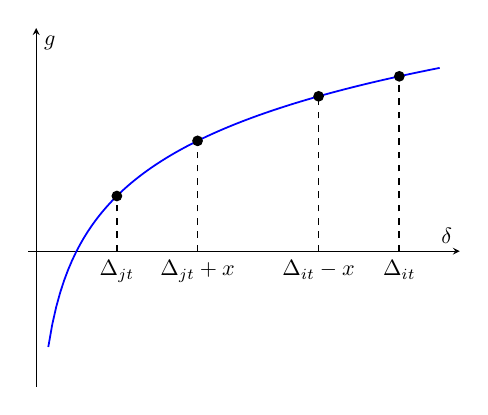
\begin{tikzpicture}[scale=0.8]
        \begin{axis}[
            domain=1:10, % Domain of the function
            samples=100, % Number of samples for the function
            axis lines=middle, % Axis lines through the middle
            xlabel={$\delta$}, % Label for x-axis
            ylabel={$g$}, % Label for y-axis
            xtick=\empty, % Remove x-axis tick marks
            ytick=\empty, % Remove y-axis tick marks
            minor tick num=1, % Number of minor ticks
            enlargelimits={abs=0.5}, % Add some space around the plot
            every axis plot/.append style={thick}, % Thicker lines for plots
        ]
            % Plot the logarithm function
            \addplot[blue, domain=0.3:10] {ln(x)};
    
            % Add points and vertical/horizontal lines
            \addplot[only marks, mark=*] coordinates {(2, 0.693) (4, 1.386) (7, 1.946) (9, 2.197)};
            \addplot[dashed] coordinates {(2,0) (2, 0.693)};
            \addplot[dashed] coordinates {(4,0) (4, 1.386)};
            \addplot[dashed] coordinates {(7,0) (7, 1.946)};
            \addplot[dashed] coordinates {(9,0) (9, 2.197)};
    
            % Add labels for the points
            \node at (axis cs:2, -0.02) [anchor=north] {$\Delta_{jt}$};
            \node at (axis cs:4, -0.02) [anchor=north] {$\Delta_{jt} + x$};
            \node at (axis cs:7, -0.02) [anchor=north] {$\Delta_{it} - x$};
            \node at (axis cs:9, -0.02) [anchor=north] {$\Delta_{it}$};
    
        \end{axis}
    \end{tikzpicture}
    
    \caption{Impact of growth increments on the compound growth rate.}
    \label{fig:log}
\end{figure}

One can interpret this as raising the base of state $s_{jt+1}$ such that the next growth increment $\delta_{jt+1}$ acts on a larger absolute value. Extending this example to a multiplicative process consisting of normally distributed increments with mean $\mu$ and standard deviation $\sigma$, the time-average growth rate without sharing converges to

\begin{gather}
    \label{eq:diversification}
    g = \mu - \frac{\sigma^2}{2}
\end{gather}

In addition to the mean $\mu$, the fluctuation term $\frac{\sigma^2}{2}$ has an outsized impact on the growth rate, as the impact of negative fluctuations on the log outweighs that of equally-sized positive fluctuations. We can easily demonstrate this since even when gaining and losing at the same rate the overall outcome will be net negative: $(1 - \epsilon_t)(1 + \epsilon_t) = 1 - \epsilon_t^2 < 1$ for any $\epsilon_t > 0$. This dynamic is referred to as \textit{variance drain} \parencite{messmore1995variance} or \textit{volatility drag} \parencite{spitznagel2021safe}. Reducing the magnitude of fluctuations is the largest lever for increasing the growth rate.  

This connects directly to the pooling result. Following \textcite{peters2022ergodicity}, with $N$ firms whose growth increments $\delta_i$ are independently drawn from the same distribution $\mathcal{N}(\mu, \sigma^2)$ and who share their absolute increments equally each period, the time-average growth rate of each firm becomes

\begin{gather}
    \label{eq:pooling_improvement}
    g = \mu - \frac{\sigma^2}{2N}
\end{gather}

As the number of firms $N$ in a conglomerate increases, the drag imposed by fluctuations decreases. In the limit $N \to \infty$ each firm is able to realize the ensemble average $\mu$ at every period. Note that the closed-form result in equation~\ref{eq:pooling_improvement} requires identical $(\mu, \sigma)$ across pool members and equal sharing weights. 

Of course there are limits to how large a conglomerate can grow, given that management cost --- particularly for coordination --- increase with scope \parencite{coase19883}. Any increase in conglomerate size raises management cost while also raising the growth rate for all member firms included. One can think of this cooperation as a hedge, or an insurance against unfavorable growth increments, the premium for which is the cost of coordination. There is a trade-off, and a conglomerate size, though certainly varying, which optimizes it. 

This concept is related to portfolio diversification but qualitatively distinct. In contrast to the latter, pooling also improves the growth rates of the entities that make up the portfolio, in addition to producing higher portfolio-level growth than diversification alone. A pure portfolio strategy solely based on diversification has an expected growth rate of as shown in Equation \ref{eq:diversification}, while conglomeration provides access to internal resource transfers, which allows for an expected growth rate as shown in \ref{eq:pooling_improvement}, which is larger than diversification for $N > 1$. We define this cooperative diversification as a cooperative arrangement that increases the time-average growth rate of each constituent unit under multiplicative dynamics, rather than merely reducing variance at the portfolio level. The  difference between pooling and standard diversification, which can be achieved by simply allowing shareholders to diversify their own portfolios across independent firms, is important. When shareholders hold diversified portfolios, they reduce their own exposure to firm-specific risk, but each firm's growth trajectory remains unchanged. If firm $i$ suffers a negative shock, $i$'s size contracts regardless of how $j$ performs. Shareholders experience the average outcome, but the firms themselves do not.

Conglomerate formation enables something qualitatively different: internal resource transfers can move capital from better-performing to worse-performing units, directly altering each unit's growth path. Note that this does not even require the worse-performing firm to suffer losses. As seen in Figure \ref{fig:log}, this mechanism also works when both constituent firms of a conglomerate experience $\delta_{it} > 1$. When $i$ underperforms while $j$ prospers, the conglomerate can channel resources to $i$, partially offsetting its decline. This is not merely risk-sharing from the perspective of a portfolio holder, but an alteration of the underlying growth dynamics of the constituent firms. 

\section{Model}
\label{sec:Model}
\subsection{Growth Process}
We employ an agent-based model to study conglomerate formation and its competitive effects.\footnote{All code, calibrated parameter values, and instructions for reproducing the simulations and figures are available in the replication package at \href{https://github.com/SimonBloethner/conglomerates}{https://github.com/SimonBloethner/conglomerates}.} This methodological choice reflects three features of the phenomenon under study. First, firm heterogeneity is essential: firms differ in their market positions, growth histories, and conglomerate memberships, and these differences drive merger decisions. A representative-agent approach would obscure the distributional dynamics central to our research questions. Second, the system exhibits strategic interdependence: firm $i$'s decision to merge with firm $j$ depends on $j$'s current conglomerate composition, which itself depends on prior merger decisions throughout the economy. This generates path-dependent dynamics where history matters for market structure. Third, the interaction of endogenous merger decisions with multiplicative growth produces emergent outcomes—market concentration, firm mobility, conglomerate size distributions—that do not reduce to analytical solutions. Hence, each firm's merger decision depends on the current state of all other firms and conglomerates, which depends on the complete history of shocks and decisions. The number of feasible merger configurations grows combinatorially with the number of firms and markets, precluding analytical tractability. In such settings, simulation is not merely a convenience but a necessity for studying how micro-level pooling incentives aggregate into macro-level market structure \parencite{axtell2025agent}. 

To investigate how growth-rate optimization influences the incentives in conglomerate formation, we set up an agent-based model with $M$ markets that are uncorrelated between each other, each containing $N$ firms. Note that introducing correlation decreases the effect sizes we obtain, but the directions remain intact. In this framework each firm's periodic state $s_{it}$, which represents its accumulated capital or the cumulative profits retained and reinvested over the firm's history, which can be seen as its size, is multiplicatively linked to its previous one. Firms face random multiplicative growth that is unique to their market. Each increment $\delta_{it}$, the gross return on capital, is drawn from a normal distribution $\mathcal{N}(\mu_m, \sigma_m^2)$ with positive ensemble average $\mu_m$.\footnote{We use $\mu_m$ to denote the drift of the log-process introduced in Section \ref{sec:Background}, with $\mathbb{E}[\delta_{it}] \approx 1 + \mu_m$ for the modest values of $\mu_m$ considered, since $\delta_{it}$ is a gross return. Parameter ranges are chosen such that the probability of negative draws is negligible.} 
\begin{gather}
    s_{i t+1} = s_{it} \delta_{it} \quad \text{with} \quad \delta_{it} \sim \mathcal{N}(\mu_m, \sigma_m^2)
\end{gather}

We model growth increments as normally distributed in order to isolate the pooling mechanism under conservative assumptions. The Gaussian distribution minimizes tail risk relative to the empirically documented Laplace distribution \textcite{stanley1996scaling,bottazzi2006explaining}, meaning our results represent a lower bound on pooling incentives. The mechanism itself depends on the concavity of the logarithm, not on the distributional form, and would be strengthened under heavier tails where large negative realizations occur more frequently, against which pooling provides the greatest protection. As explained in section \ref{sec:Background}, in multiplicative processes one is not just maximizing for the ensemble average $\mu_m$, but for the growth rate $g$. Hence, a higher scale $\sigma_m$ decreases the growth rate, through the volatility tax. A natural concern is that focusing on variance reduction ignores the risk-return tradeoff: markets with higher risk often offer higher expected returns \parencite{cont2001empirical}. We explicitly incorporate this by modeling a positive correlation between market-level means $\mu_m$ and standard deviations $\sigma_m$. Firms thus face a genuine choice between high-$\mu$, high-$\sigma$ markets and low-$\mu$, low-$\sigma$ markets. The time-average growth rate $g = \mu - \frac{\sigma^2}{2}$ captures this tradeoff, since a market with $\mu = 0.12$ and $\sigma = 0.3$ yields $g = 0.075$, while one with $\mu = 0.08$ and $\sigma = 0.1$ yields $g = 0.075$. Even though these two exhibit identical growth rates they offer different risk profiles. Pooling allows firms to access high-$\mu$ markets while mitigating their variance penalty. This specification reflects well-documented heterogeneity across industries. Cross-sectional analysis of industry returns shows that high-growth sectors exhibit substantially greater volatility: technology and biotechnology sectors display volatility two to five times higher than defensive sectors such as utilities and consumer staples \parencite{fama1992cross,fama1993common}. At the firm level, \textcite{bottazzi2006explaining} confirm that while growth-rate distributions share common properties across sectors, their variance differs systematically by industry characteristics. \textcite{klepper1996entry,klepper1997industry} document that emerging industries experience entry and exit rates several times higher than mature industries, generating greater firm-level turbulence. International evidence reinforces this pattern: emerging equity markets exhibit both higher expected returns and higher volatility than developed markets \parencite{bekaert1997emerging}. By drawing market parameters from correlated distributions, we capture this cross-sectional variation while maintaining tractability. \\
Each firm thus realizes an absolute period gain of $\Delta_{it} = s_{it} \delta_{it} - s_{it}$. For any firm not part of a conglomerate this will also be their period profit $\Pi_{it} = \Delta_{it}$. Firms in conglomerates $C$ pool an amount $\alpha \Delta_{it}$, which flows into the conglomerate's period pool $\Omega_{ct} = \sum_{i \in c} \alpha \Delta_{it}$, with $\alpha \in [0, 1]$. The growth process is multiplicative at the shock level but additive at the accounting level. Firms experience multiplicative shocks to size, but pooling operates on realized absolute gains, which are naturally additive. The pooling mechanism models profit-sharing within conglomerates. When members pool a fraction $\alpha$ of their period profits, resources flow from more profitable to less profitable divisions. This reflects the institutional reality that internal capital markets redistribute realized resources rather than growth rates themselves \parencite{gertner1994internal,stein1997internal}. As conglomerates grow, management costs increase.\footnote{We abstract from fixed costs and increasing returns to scale, not because they are unimportant, but because they create merger incentives that are already well understood. By excluding them, we isolate the contribution of resource pooling under multiplicative dynamics as a distinct driver of conglomerate formation.} We model these using four different functional forms:

\begin{gather}
    \label{eq:power_law}
    \Phi (O_c) = b_{0p} |O_c| ^ {b_{1p}}
\end{gather}
\begin{gather}
    \label{eq:linear}
    \Phi (O_c) = b_{0l} + b_{1l} |O_c|
\end{gather}
\begin{gather}
    \label{eq:quadratic}
    \Phi (O_c) = b_{0q} + b_{1q} |O_c| + b_{2q} |O_c|^2 
\end{gather}
\begin{gather}
    \label{eq:exponential}
    \Phi (O_c) = b_{0e} e^{b_{1e} |O_c|}
\end{gather}

The parameters $b$ are management cost scaling hyperparameters for the power law ($p$), linear ($l$), quadratic ($q$), and exponential ($e$) cost functions. $O_c \in \mathcal{M}$ is the set of markets out of all markets $\mathcal{M}$ that a conglomerate operates in. The literature on management diseconomies provides theoretical foundations \parencite{coase19883,williamson1967hierarchical} but limited empirical guidance on the precise functional form of coordination costs. \textcite{williamson1967hierarchical} suggests that diseconomies arise from communication distortion, bureaucratic insularity, and incentive limits, but these mechanisms could plausibly generate linear, convex, or even initially concave cost structures depending on organizational form and industry context. \textcite{canback2006diseconomies} find empirically that diseconomies and scale economies tend to offset each other, making the functional form difficult to identify directly. Given this theoretical and empirical ambiguity, we compare four functional forms representing the main possibilities: power law (initially concave), linear, quadratic (convex), and exponential (strongly convex). Rather than treating this as purely a robustness check, we treat the cost structure as a parameter of interest: while the direction of pooling effects is robust across specifications, the magnitude varies substantially, which has implications for optimal conglomerate size. We calibrate the cost function parameters such that all four specifications yield equivalent costs at a conglomerate size of 40 members, which represents a mid-range conglomerate in our setup with $M \in \{50, 100, 150\}$ markets. We also vary these parameters around these baseline values across simulations to ensure our results are not driven by a particular calibration choice. Once computed, this cost factor scales the cost according to conglomerate's total capital $\sum_{i \in c} s_{it}$ such that the pool size is given by

\begin{gather}
    \Omega_{ct} = \sum_{i \in c} \alpha \Delta_{it} -  \Phi (O_c) \sum_{i \in c} s_{it}
    \label{eq:comp_pool}
\end{gather}
This pool will be shared equally, determining a member's profit by
$\Pi_{it} = (1 - \alpha) \Delta_{it} + \frac{\Omega_{ct}}{|O_{c_i}|}$\,. Consequently, any firm's next state is given by $s_{it+1} = s_{it} + \Pi_{it}$. We can measure market concentration through each firm's share of total capital within its market:

$$ \frac{s_{it}}{\sum_{j \in m_i} s_{jt}}. $$

This yields capital share distributions rather than conventional revenue-based market shares. This approach is well-grounded in industrial organization theory. The \textcite{kreps1983quantity} framework demonstrates that when firms first choose production capacity and then compete on price, the equilibrium outcome equals Cournot competition—capacity determined by capital investment is the strategically relevant variable, with sales as the subsequent outcome. \textcite{dixit1980role} reinforces this logic through entry deterrence theory: a firm's capital stock represents a credible commitment that shapes post-entry competition, making accumulated investment the determinant of sustainable competitive position. \textcite{sutton1991sunk} extends this insight, showing that in industries with significant sunk costs, there exists a lower bound on concentration determined by the scale of capital investments required for viable operation.

Empirically, asset-based concentration measures are standard practice in several domains. \textcite{scitovsky1955economic} explicitly discusses choosing between ``employment, sales, value added, value of total assets, and 'net capital assets''' as concentration measures, noting that asset-based measures may capture different aspects of market power than sales-based measures. \textcite{dang2018measuring} survey 100 empirical articles and find that total assets ranks alongside sales as among the most common firm size proxies, with the appropriate choice depending on context. \textcite{kwon2024100} use both asset share and sales share as parallel concentration measures in their century-long study of U.S. corporate concentration, finding correlation exceeding $0.99$ between alternative measures. In banking, the Federal Reserve uses deposits—a liability-side capital measure—rather than revenue for merger concentration analysis, as deposits proxy for lending capacity. The European Central Bank similarly reports banking concentration using total assets. In electricity markets, FERC calculates merger HHIs based on generation capacity shares rather than revenue \parencite{roach2002measuring}. In international trade, UNCTAD ranks multinational enterprises by foreign assets, and gravity models routinely use FDI stocks as measures of market presence \parencite{ramondo2013trade}. The theoretical rationale is consistent across these applications: accumulated capital represents credible commitment and determines cost structure, while sales fluctuate with transitory demand conditions. For analyzing market concentration dynamics, capital-based measures capture sustainable competitive position rather than period-specific outcomes.

\subsection{Merging and Splitting}

At the beginning of every time step $t$ each firm $i \in {1, \ldots, MN}$  gets a chance to choose another with probability $p$. If successful, it will select a random other firm $j$, among the remaining $(M \times N) - 1$ firms. 
Consistent with the convention that conglomerate mergers are neither horizontal nor vertical, we restrict conglomerates to operate at most one firm per market. This prevents within-conglomerate horizontal overlap by construction. Hence, conglomeration is only \textit{feasible} if firm $j$ and $i$: 

\begin{enumerate}
    \item don't operate in the same market $(m_i \neq m_j)$
    \item are not part of a conglomerate that operates in a market in which the other firm, or the conglomerate which it is part of operates in $(O_{c_i} \cap O_{c_j} = \emptyset)$
\end{enumerate}

We assume that if both firms are in conglomerates that these will merge as well. After confirming \textit{feasibility}, merging firms determine \textit{desirability}, meaning that they would both benefit from joining forces.
They do so by comparing the realized pool $\Omega$ size over the last $l$ periods, against a ``synthetic'' pool $\hat{\Omega}$ size if they had merged.

Specifically, firms compute $\hat{\Omega}$ by applying the pooling formula \ref{eq:comp_pool} to their combined historical increments $\{ \Delta_{it}, \Delta_{jt} \}_{t=t_l}$ over the lookback period $l$, using the management cost that would apply to the combined entity. This assumes firms have access to each other's historical performance data, which could be interpreted as the due diligence process preceding merger negotiations. If $\hat{\Omega} > \Omega$ the merger will be implemented, since the combined entity generates a larger resource pool than the separate arrangements. We adopt a backward-looking heuristic in the spirit of \textcite{simon1955behavioral}: firms cannot condition on future shocks and must estimate merger desirability from realized history. Since pool resources are distributed equally among members, an increase in the total pool translates into increased per-member transfers provided the pool grows faster than membership.

After being in a conglomerate for at least $l$ periods, each firm evaluates its performance within it by comparing its growth rate $g_{i(t-l):t}$ being part of the conglomerate against the potential rate $\hat{g}_{i(t-l):t}$ it had realized, had it remained outside. Upon being worse off, a firm exits the conglomerate and continues to operate alone until it gets the chance to join another conglomerate. Importantly, our merger evaluation and exit decisions are based on historical performance over the lookback window $l$, which are used as a guide for expected future performance. This reflects information constraints: firms observe realized outcomes but do not know future shock realizations or other firms' future decisions. All empirical evaluation of business decisions necessarily relies on realized historical data. Our lookback window $l$ represents the information firms use to assess merger desirability and conglomerate performance, analogous to the historical performance data used in real merger due diligence. The assumption is not that firms are myopic in their objectives, but that they are informationally constrained: they seek to maximize long-run growth but must estimate which arrangements achieve this using only past performance. Thus, our decision rules reflect bounded rationality in the sense of \textcite{simon1955behavioral}: firms use simple heuristics based on observable historical performance rather than computing optimal forward-looking strategies that would require heavy assumptions and knowledge of future shock distributions and other firms' strategies. Given that our focus is on the pooling mechanism rather than strategic merger bargaining, the heuristic provides a tractable and empirically plausible alternative. \\

To summarize the model flow: each period, firms receive random opportunities to initiate mergers. Feasible mergers are those where the parties operate in non-overlapping markets. Desirable mergers are those where historical evidence suggests the combined pool would outperform the separate arrangements. After merger decisions, conglomerates compute their period pools, distribute profits, and update firm states. Finally, members evaluate their conglomerate membership against counterfactual standalone performance and exit if the conglomerate reduces their growth rate. The full formalization of the model can be seen in algorithm \ref{alg:rand_growth}. \par

\vspace{0.8cm}


\begin{algorithm}[H]
    \label{alg:rand_growth}
    \For{$t$ in $T$}{
      \ForEach{$i$ $\in$ $N \times M$}{
        Merge with $j$ if $(m_i \neq m_j)$ and $(O_{c_i} \cap O_{c_j} = \emptyset)$ and $\hat{\Omega} > \Omega$  
      }
      \ForEach{$c \in C$}{
        $\Omega_{ct} = \sum_{i \in c} \alpha \Delta_{it} -  \Phi (O_c) \sum_{i \in c} s_{it}$ \\
        \ForEach{$i \in c$}{$\Pi_{it} = (1 - \alpha) \Delta_{it} + \frac{\Omega_{ct}}{|O_c|}$} 
      }
      \ForEach{$i \notin \bigcup_{c \in C}$}{$\Pi_{it} = \Delta_{it}$}   
      
      \ForEach{$i \in \bigcup_{c \in C}$}{
        Exit $c$ if $\hat{g}_{i(t-l):t} > g_{i(t-l):t}$
      }

    }
    \caption{Model flow}
\end{algorithm}


\section{Results}
\label{sec:Results}
We implemented the model in Python with extensive robustness testing. For each hyperparameter in Table \ref{tab:model_params}, we construct scenarios that vary a particular hyperparameter while holding others at baseline; this yields 54 scenarios in total. We do not run the full Cartesian product, as this would not be computationally feasible. Within each scenario we vary the pooling rate $\alpha$ across $[0,0.5]$ in steps of 0.02 (26 levels), and run 50 Monte Carlo replications per cell. This produces 70,200 simulations.

\begin{table}[h]
    \centering
    \begin{tabular}{|c|c|}
    \hline
    \textbf{Parameter} & \textbf{Value} \\
    \hline
    $M$ & \{50, 100, 150\} \\
    $N$ & \{50, 100, 150\} \\
    $T$ & 10000 \\
    $l$ & \{10, 50, 100\} \\
    $p$ & \{0.01, 0.05, 0.1\} \\
    $\Phi$ & {$l, e, p, q$ } \\
    $\alpha$ & $\left[0, 0.5 \right]$ \\
    \hline
    \end{tabular}
    \caption{Model Parameters and their values}
    \label{tab:model_params}
\end{table}

Given the high-dimensionality of our results, we estimate several panel regressions, controlling for the counterfactual heterogeneity to isolate the effect of our variable of interest $\alpha$ on the question outlined in Section \ref{sec:Background}. Table \ref{tab:dynamics} shows the impact of a change in pooling on the per-period average conglomerate size, number of conglomerates, mergers, and exits (defined as a firm leaving a conglomerate). Importantly, we estimate a quadratic model, as well as interactive terms with structural market parameters and the lookback period, to capture any non-linear effects. These interactions are mostly substantively meaningful and statistically significant, indicating that pooling increases all metrics up to a point before reducing them. Mergers and exits scale together with $\alpha$ at near-identical rates (coefficients 582.88 vs 583.33), consistent with stable conglomerate formation in which entry and exit balance rather than runaway concentration. Additionally, we observe that increasing $\alpha$ produces more conglomerates with fewer members on average, indicating that pooling promotes a larger number of smaller conglomerates rather than the formation of a few dominant ones. These effects are, however, not homogenous across cost structures. Table \ref{tab:dynamics} also reports interaction terms to assess whether the pooling effect is moderated by model parameters. The interaction $l \times \alpha$ reveals that longer lookback windows produce larger but more stable conglomerates: firms with more historical data form slightly larger entities ($\beta = 0.062$) with less merger and exit churn ($\beta = -5.95$). The market and firm dimensions ($M \times \alpha, N \times \alpha$) show near-symmetric effects, expanding the number of conglomerates without altering their average size or the qualitative relationship between pooling and market dynamics. These results indicate the qualitative pooling effects are stable across the parameter ranges examined, with the lookback window primarily affecting the speed of conglomerate adjustment rather than its direction. To demonstrate these effects more clearly, Figure \ref{fig:metrics} shows that power law cost scaling leads to comparatively larger, but fewer conglomerates. It also produces merging and exit patterns that are much less dynamic than those of the rest of the cost structures. Since costs scale initially slower in the power law case, conglomerates can form more reliably, lowering the number of exits and consequently also the number of firms able to join new ones. 

\begin{table}[htbp]
    \centering
    \renewcommand{\arraystretch}{1.3}
    \begin{tabular}{lcccc}
        \toprule
        & (1) & (2) & (3) & (4) \\
        & Avg.\ Members & Num.\ Conglomerates & Mergers & Exits \\
        \midrule
        $\alpha$ 
            & 8.01*** & 2407.60*** & 582.88*** & 583.33*** \\
            & (0.02)  & (8.04)     & (0.64)    & (0.66)    \\

        $\alpha^2$ 
            & -12.87*** & -7857.29*** & -483.93*** & -482.74*** \\
            & (0.02)    & (7.12)      & (0.57)     & (0.58)     \\

        $l \times \alpha$ 
            & 0.0623*** & 18.1266*** & -5.9509*** & -5.9591*** \\
            & (0.0001)  & (0.0282)   & (0.0023)   & (0.0023)   \\

        $M \times \alpha$ 
            & 0.0029*** & 6.4084*** & -0.2712*** & -0.2771*** \\
            & (0.0001)  & (0.0495)  & (0.0040)   & (0.0040)   \\

        $N \times \alpha$ 
            & -0.0000   & 6.3513*** & -0.2756*** & -0.2816*** \\
            & (0.0001)  & (0.0495)  & (0.0040)   & (0.0040)   \\

        \midrule
        Obs.  & 14040000 & 14040000 & 14040000 & 14040000 \\
        R$^{2}$ & 0.72 & 0.64 & 0.57 & 0.56 \\
        \bottomrule
        \multicolumn{5}{l}{\footnotesize \textit{Note:} Standard errors in parentheses.} \\
        \multicolumn{5}{l}{\footnotesize $^{*}p<0.1$; $^{**}p<0.05$; $^{***}p<0.01$} \\
    \end{tabular}
    \caption{Panel regression results showing how pooling affects conglomerate size, number of conglomerates, number of mergers, and number of exits. Regression uses one Monte Carlo replication per scenario $ \times \alpha$ cell ($54 \times 26 \times 10{,}000 = 14{,}040{,}000$ observations). Standard errors are pooled-OLS and unadjusted for serial correlation within cells. All specifications include cost-type fixed effects and controls for $M$, $N$, and $p$.}
    \label{tab:dynamics}
\end{table}



% Metrics by cooperation level across cost structures
% This file is \input into the main document

\begin{figure}[htbp]
\centering
\begin{tikzpicture}
\begin{groupplot}[
    group style={
        group size=2 by 2,
        horizontal sep=1.5cm,
        vertical sep=1.5cm
    },
    width=0.45\textwidth,
    height=0.35\textwidth,
    xmin=0,
    xmax=0.5,
    grid=both,
    tick label style={font=\small},
    label style={font=\small},
    scaled ticks=false,
    xticklabel style={
        /pgf/number format/.cd,
            fixed,
            fixed zerofill,
            precision=2,
    },
]

% -------- Metric 0 (top left) --------
\nextgroupplot[title={Conglomerate Size}, legend to name=metricslegend, legend columns=4]
% ===== Metric 0, All cost types =====

% Cost type 0 (Linear)
\addplot[name path=med0, cost0, thick]
table[col sep=comma, x=alpha, y=median]{figures/plots/m0_cost0.csv};

\addplot[name path=low0, draw=none, forget plot]
table[col sep=comma, x=alpha, y=q25]{figures/plots/m0_cost0.csv};

\addplot[name path=high0, draw=none, forget plot]
table[col sep=comma, x=alpha, y=q75]{figures/plots/m0_cost0.csv};

\addplot[cost0!30, fill opacity=0.3, forget plot] fill between[of=low0 and high0];

% Cost type 1 (Quadratic)
\addplot[name path=med1, cost1, thick]
table[col sep=comma, x=alpha, y=median]{figures/plots/m0_cost1.csv};

\addplot[name path=low1, draw=none, forget plot]
table[col sep=comma, x=alpha, y=q25]{figures/plots/m0_cost1.csv};

\addplot[name path=high1, draw=none, forget plot]
table[col sep=comma, x=alpha, y=q75]{figures/plots/m0_cost1.csv};

\addplot[cost1!30, fill opacity=0.3, forget plot] fill between[of=low1 and high1];

% Cost type 2 (Power law)
\addplot[name path=med2, cost2, thick]
table[col sep=comma, x=alpha, y=median]{figures/plots/m0_cost2.csv};

\addplot[name path=low2, draw=none, forget plot]
table[col sep=comma, x=alpha, y=q25]{figures/plots/m0_cost2.csv};

\addplot[name path=high2, draw=none, forget plot]
table[col sep=comma, x=alpha, y=q75]{figures/plots/m0_cost2.csv};

\addplot[cost2!30, fill opacity=0.3, forget plot] fill between[of=low2 and high2];

% Cost type 3 (Exponential)
\addplot[name path=med3, cost3, thick]
table[col sep=comma, x=alpha, y=median]{figures/plots/m0_cost3.csv};

\addplot[name path=low3, draw=none, forget plot]
table[col sep=comma, x=alpha, y=q25]{figures/plots/m0_cost3.csv};

\addplot[name path=high3, draw=none, forget plot]
table[col sep=comma, x=alpha, y=q75]{figures/plots/m0_cost3.csv};

\addplot[cost3!30, fill opacity=0.3, forget plot] fill between[of=low3 and high3];

\legend{Linear, Quadratic, Power law, Exponential}


% -------- Metric 1 (top right) --------
\nextgroupplot[title={Conglomerate Count}]
% ===== Metric 1, All cost types =====

% Cost type 0 (Linear)
\addplot[name path=med0, cost0, thick]
table[col sep=comma, x=alpha, y=median]{figures/plots/m1_cost0.csv};

\addplot[name path=low0, draw=none, forget plot]
table[col sep=comma, x=alpha, y=q25]{figures/plots/m1_cost0.csv};

\addplot[name path=high0, draw=none, forget plot]
table[col sep=comma, x=alpha, y=q75]{figures/plots/m1_cost0.csv};

\addplot[cost0!30, fill opacity=0.3, forget plot] fill between[of=low0 and high0];

% Cost type 1 (Quadratic)
\addplot[name path=med1, cost1, thick]
table[col sep=comma, x=alpha, y=median]{figures/plots/m1_cost1.csv};

\addplot[name path=low1, draw=none, forget plot]
table[col sep=comma, x=alpha, y=q25]{figures/plots/m1_cost1.csv};

\addplot[name path=high1, draw=none, forget plot]
table[col sep=comma, x=alpha, y=q75]{figures/plots/m1_cost1.csv};

\addplot[cost1!30, fill opacity=0.3, forget plot] fill between[of=low1 and high1];

% Cost type 2 (Power law)
\addplot[name path=med2, cost2, thick]
table[col sep=comma, x=alpha, y=median]{figures/plots/m1_cost2.csv};

\addplot[name path=low2, draw=none, forget plot]
table[col sep=comma, x=alpha, y=q25]{figures/plots/m1_cost2.csv};

\addplot[name path=high2, draw=none, forget plot]
table[col sep=comma, x=alpha, y=q75]{figures/plots/m1_cost2.csv};

\addplot[cost2!30, fill opacity=0.3, forget plot] fill between[of=low2 and high2];

% Cost type 3 (Exponential)
\addplot[name path=med3, cost3, thick]
table[col sep=comma, x=alpha, y=median]{figures/plots/m1_cost3.csv};

\addplot[name path=low3, draw=none, forget plot]
table[col sep=comma, x=alpha, y=q25]{figures/plots/m1_cost3.csv};

\addplot[name path=high3, draw=none, forget plot]
table[col sep=comma, x=alpha, y=q75]{figures/plots/m1_cost3.csv};

\addplot[cost3!30, fill opacity=0.3, forget plot] fill between[of=low3 and high3];


% -------- Metric 2 (bottom left) --------
\nextgroupplot[title={Periodic Mergers}, xlabel={$\alpha$ (Pooling Rate)}]
% ===== Metric 2, All cost types =====

% Cost type 0 (Linear)
\addplot[name path=med0, cost0, thick]
table[col sep=comma, x=alpha, y=median]{figures/plots/m2_cost0.csv};

\addplot[name path=low0, draw=none, forget plot]
table[col sep=comma, x=alpha, y=q25]{figures/plots/m2_cost0.csv};

\addplot[name path=high0, draw=none, forget plot]
table[col sep=comma, x=alpha, y=q75]{figures/plots/m2_cost0.csv};

\addplot[cost0!30, fill opacity=0.3, forget plot] fill between[of=low0 and high0];

% Cost type 1 (Quadratic)
\addplot[name path=med1, cost1, thick]
table[col sep=comma, x=alpha, y=median]{figures/plots/m2_cost1.csv};

\addplot[name path=low1, draw=none, forget plot]
table[col sep=comma, x=alpha, y=q25]{figures/plots/m2_cost1.csv};

\addplot[name path=high1, draw=none, forget plot]
table[col sep=comma, x=alpha, y=q75]{figures/plots/m2_cost1.csv};

\addplot[cost1!30, fill opacity=0.3, forget plot] fill between[of=low1 and high1];

% Cost type 2 (Power law)
\addplot[name path=med2, cost2, thick]
table[col sep=comma, x=alpha, y=median]{figures/plots/m2_cost2.csv};

\addplot[name path=low2, draw=none, forget plot]
table[col sep=comma, x=alpha, y=q25]{figures/plots/m2_cost2.csv};

\addplot[name path=high2, draw=none, forget plot]
table[col sep=comma, x=alpha, y=q75]{figures/plots/m2_cost2.csv};

\addplot[cost2!30, fill opacity=0.3, forget plot] fill between[of=low2 and high2];

% Cost type 3 (Exponential)
\addplot[name path=med3, cost3, thick]
table[col sep=comma, x=alpha, y=median]{figures/plots/m2_cost3.csv};

\addplot[name path=low3, draw=none, forget plot]
table[col sep=comma, x=alpha, y=q25]{figures/plots/m2_cost3.csv};

\addplot[name path=high3, draw=none, forget plot]
table[col sep=comma, x=alpha, y=q75]{figures/plots/m2_cost3.csv};

\addplot[cost3!30, fill opacity=0.3, forget plot] fill between[of=low3 and high3];


% -------- Metric 3 (bottom right) --------
\nextgroupplot[title={Periodic Exits}, xlabel={$\alpha$ (Pooling Rate)}]
% ===== Metric 3, All cost types =====

% Cost type 0 (Linear)
\addplot[name path=med0, cost0, thick]
table[col sep=comma, x=alpha, y=median]{figures/plots/m3_cost0.csv};

\addplot[name path=low0, draw=none, forget plot]
table[col sep=comma, x=alpha, y=q25]{figures/plots/m3_cost0.csv};

\addplot[name path=high0, draw=none, forget plot]
table[col sep=comma, x=alpha, y=q75]{figures/plots/m3_cost0.csv};

\addplot[cost0!30, fill opacity=0.3, forget plot] fill between[of=low0 and high0];

% Cost type 1 (Quadratic)
\addplot[name path=med1, cost1, thick]
table[col sep=comma, x=alpha, y=median]{figures/plots/m3_cost1.csv};

\addplot[name path=low1, draw=none, forget plot]
table[col sep=comma, x=alpha, y=q25]{figures/plots/m3_cost1.csv};

\addplot[name path=high1, draw=none, forget plot]
table[col sep=comma, x=alpha, y=q75]{figures/plots/m3_cost1.csv};

\addplot[cost1!30, fill opacity=0.3, forget plot] fill between[of=low1 and high1];

% Cost type 2 (Power law)
\addplot[name path=med2, cost2, thick]
table[col sep=comma, x=alpha, y=median]{figures/plots/m3_cost2.csv};

\addplot[name path=low2, draw=none, forget plot]
table[col sep=comma, x=alpha, y=q25]{figures/plots/m3_cost2.csv};

\addplot[name path=high2, draw=none, forget plot]
table[col sep=comma, x=alpha, y=q75]{figures/plots/m3_cost2.csv};

\addplot[cost2!30, fill opacity=0.3, forget plot] fill between[of=low2 and high2];

% Cost type 3 (Exponential)
\addplot[name path=med3, cost3, thick]
table[col sep=comma, x=alpha, y=median]{figures/plots/m3_cost3.csv};

\addplot[name path=low3, draw=none, forget plot]
table[col sep=comma, x=alpha, y=q25]{figures/plots/m3_cost3.csv};

\addplot[name path=high3, draw=none, forget plot]
table[col sep=comma, x=alpha, y=q75]{figures/plots/m3_cost3.csv};

\addplot[cost3!30, fill opacity=0.3, forget plot] fill between[of=low3 and high3];


\end{groupplot}

% Add legend at the bottom of the entire figure
\node at ($(group c1r2.south)!0.5!(group c2r2.south) - (0,1.5cm)$) [anchor=north] {%
    \pgfplotslegendfromname{metricslegend}%
};

\end{tikzpicture}
\label{fig:metrics}
\caption{Conglomerate metrics by pooling level across cost structures. The solid line indicates the median and the shaded region is between the 25th and 75th percentile.}
\end{figure}


To further examine the impact of mergers on the competitive landscape and to deepen our understanding of the role that management cost play, we fit a polynomial of degree two in a panel setting in Equation~\ref{eq:reg_model} to the relation between conglomerate size and average capital share of firms within a given conglomerate within each simulation. Afterwards we aggregate these results per hyperparameter. 
\begin{gather}
    \label{eq:reg_model}
    \bar{m}_{ct} = \beta_{0t} + \beta_{1t} |O_{ct}| + \beta_{2t} |O_{ct}|^2
\end{gather}
We calculate the average market share for a conglomerate as

\begin{gather}
       \bar{m}_{ct} = \frac{1}{|c|} \sum_{i \in c} \frac{s_{it}}{\sum_{j \in m_i} s_{jt}}
   \end{gather}

The regression in equation \ref{eq:reg_model} is estimated by pooled OLS across all scenarios and Monte Carlo replications, with cost-type fixed effects and controls for the number of markets $M$, the number of firms per market $N$, and the matching probability $p$. Figure \ref{fig:panel_poly} reports the medians of $\beta_1$ and $\beta_2$ across Monte Carlo replications for each cost type and $\alpha$ level, with shading indicating the 25th--75th percentile range. 

We expect the conglomerate size to have a positive impact on the average capital share ($\beta_{1t} > 0$). However, we expect management costs to impose a drag high enough to negatively influence the average capital share ($\beta_{2t} < 0$). Figure \ref{fig:panel_poly} shows that this hypothesis holds only to a certain extent. Initially, for all cost types except the power law one, we see $\beta_1 > 0 > \beta_2$. As we increase the level of pooling, this relation flips, however, the magnitude is much less pronounced, since the scale of the two estimates differs by an order of magnitude. The reversal of $\beta_1$ at higher pooling rates reflects the interaction between pooling intensity and coordination costs. At low $\alpha$, larger conglomerates enjoy greater variance reduction, conferring a growth advantage over smaller ones. As $\alpha$ increases, however, coordination costs, which scale with conglomerate size, increasingly offset the pooling benefit. Beyond a threshold, smaller conglomerates achieve a more favorable trade-off between variance reduction and coordination overhead, reversing the size-advantage relationship. The ordering of the sign reversal across cost structures is informative. Power law costs, which scale initially slowly, permit the formation of larger conglomerates (Figure \ref{fig:metrics}). These larger entities saturate the pooling benefit at lower $\alpha$, causing the size-advantage relationship to reverse earliest. Exponential costs, by contrast, constrain conglomerate size, meaning that even at moderate pooling rates, additional members still contribute net growth benefits — the size advantage persists to higher values of $\alpha$ before coordination costs dominate. This ordering confirms that the sign reversal reflects the interaction between conglomerate scale and coordination costs: where conglomerates can grow large, the diminishing marginal benefit of additional members manifests sooner. The convergence of both $\beta_1$ and $\beta_2$ toward zero at high $\alpha$ reflects the compression of the capital share distribution among conglomerate members as pooling intensity increases. This is a direct consequence of a decrease in the variability and scale of capital share inequality. In short, the size-advantage of larger conglomerates is real at low pooling rates and disappears or reverses at high pooling rates, with the threshold determined by how steeply coordination costs scale.

\begin{figure}[htbp]
  \centering
    \begin{tikzpicture}
        \begin{groupplot}[
            group style={
                group size=2 by 1,
                horizontal sep=2cm
            },
            width=0.45\textwidth,
            height=0.35\textwidth,
            xmin=0,
            xmax=0.5,
            xlabel={$\alpha$ (Profit Sharing)},
            grid=both,
            tick label style={font=\small},
            label style={font=\small},
            scaled ticks=false,
            xticklabel style={/pgf/number format/fixed, /pgf/number format/precision=2},
            yticklabel style={/pgf/number format/fixed, /pgf/number format/precision=3},
            % Define plot styles for cost types
            /pgfplots/cost0/.style={color=cost0},
            /pgfplots/cost1/.style={color=cost1},
            /pgfplots/cost2/.style={color=cost2},
            /pgfplots/cost3/.style={color=cost3},
        ]

        % Left panel: β₁
            \nextgroupplot[ylabel={$\beta_1$ (Linear Coefficient)}, legend to name=polylegend, legend columns=4]
              % Beta1 plot - all cost types

  % Cost type 0 (Linear)
  \addplot[name path=med0, cost0, thick, mark=*, mark size=1.5pt]
  table[col sep=comma, x=alpha, y=median]{figures/plots/poly_beta1_cost0.csv};

  \addplot[name path=low0, draw=none, forget plot]
  table[col sep=comma, x=alpha, y=q25]{figures/plots/poly_beta1_cost0.csv};

  \addplot[name path=high0, draw=none, forget plot]
  table[col sep=comma, x=alpha, y=q75]{figures/plots/poly_beta1_cost0.csv};

  \addplot[cost0!30, forget plot] fill between[of=low0 and high0];

  % Cost type 1 (Quadratic)
  \addplot[name path=med1, cost1, thick, mark=*, mark size=1.5pt]
  table[col sep=comma, x=alpha, y=median]{figures/plots/poly_beta1_cost1.csv};

  \addplot[name path=low1, draw=none, forget plot]
  table[col sep=comma, x=alpha, y=q25]{figures/plots/poly_beta1_cost1.csv};

  \addplot[name path=high1, draw=none, forget plot]
  table[col sep=comma, x=alpha, y=q75]{figures/plots/poly_beta1_cost1.csv};

  \addplot[cost1!30, forget plot] fill between[of=low1 and high1];

  % Cost type 2 (Power law)
  \addplot[name path=med2, cost2, thick, mark=*, mark size=1.5pt]
  table[col sep=comma, x=alpha, y=median]{figures/plots/poly_beta1_cost2.csv};

  \addplot[name path=low2, draw=none, forget plot]
  table[col sep=comma, x=alpha, y=q25]{figures/plots/poly_beta1_cost2.csv};

  \addplot[name path=high2, draw=none, forget plot]
  table[col sep=comma, x=alpha, y=q75]{figures/plots/poly_beta1_cost2.csv};

  \addplot[cost2!30, forget plot] fill between[of=low2 and high2];

  % Cost type 3 (Exponential)
  \addplot[name path=med3, cost3, thick, mark=*, mark size=1.5pt]
  table[col sep=comma, x=alpha, y=median]{figures/plots/poly_beta1_cost3.csv};

  \addplot[name path=low3, draw=none, forget plot]
  table[col sep=comma, x=alpha, y=q25]{figures/plots/poly_beta1_cost3.csv};

  \addplot[name path=high3, draw=none, forget plot]
  table[col sep=comma, x=alpha, y=q75]{figures/plots/poly_beta1_cost3.csv};

  \addplot[cost3!30, forget plot] fill between[of=low3 and high3];

  % Add horizontal line at y=0
  \addplot[black, dashed, forget plot] coordinates {(0,0) (0.5,0)};

  \legend{Linear, Quadratic, Power law, Exponential}

            % Right panel: β₂
            \nextgroupplot[ylabel={$\beta_2$ (Quadratic Coefficient)}]
            % Beta2 plot - all cost types

  % Cost type 0 (Linear)
  \addplot[name path=med0, cost0, thick, mark=*, mark size=1.5pt]
  table[col sep=comma, x=alpha, y=median]{figures/plots/poly_beta2_cost0.csv};

  \addplot[name path=low0, draw=none, forget plot]
  table[col sep=comma, x=alpha, y=q25]{figures/plots/poly_beta2_cost0.csv};

  \addplot[name path=high0, draw=none, forget plot]
  table[col sep=comma, x=alpha, y=q75]{figures/plots/poly_beta2_cost0.csv};

  \addplot[cost0!30, forget plot] fill between[of=low0 and high0];

  % Cost type 1 (Quadratic)
  \addplot[name path=med1, cost1, thick, mark=*, mark size=1.5pt]
  table[col sep=comma, x=alpha, y=median]{figures/plots/poly_beta2_cost1.csv};

  \addplot[name path=low1, draw=none, forget plot]
  table[col sep=comma, x=alpha, y=q25]{figures/plots/poly_beta2_cost1.csv};

  \addplot[name path=high1, draw=none, forget plot]
  table[col sep=comma, x=alpha, y=q75]{figures/plots/poly_beta2_cost1.csv};

  \addplot[cost1!30, forget plot] fill between[of=low1 and high1];

  % Cost type 2 (Power law)
  \addplot[name path=med2, cost2, thick, mark=*, mark size=1.5pt]
  table[col sep=comma, x=alpha, y=median]{figures/plots/poly_beta2_cost2.csv};

  \addplot[name path=low2, draw=none, forget plot]
  table[col sep=comma, x=alpha, y=q25]{figures/plots/poly_beta2_cost2.csv};

  \addplot[name path=high2, draw=none, forget plot]
  table[col sep=comma, x=alpha, y=q75]{figures/plots/poly_beta2_cost2.csv};

  \addplot[cost2!30, forget plot] fill between[of=low2 and high2];

  % Cost type 3 (Exponential)
  \addplot[name path=med3, cost3, thick, mark=*, mark size=1.5pt]
  table[col sep=comma, x=alpha, y=median]{figures/plots/poly_beta2_cost3.csv};

  \addplot[name path=low3, draw=none, forget plot]
  table[col sep=comma, x=alpha, y=q25]{figures/plots/poly_beta2_cost3.csv};

  \addplot[name path=high3, draw=none, forget plot]
  table[col sep=comma, x=alpha, y=q75]{figures/plots/poly_beta2_cost3.csv};

  \addplot[cost3!30, forget plot] fill between[of=low3 and high3];

  % Add horizontal line at y=0
  \addplot[black, dashed, forget plot] coordinates {(0,0) (0.5,0)};

        \end{groupplot}

        % Place legend below both plots, centered
        \node at ($(group c1r1.south)!0.5!(group c2r1.south) - (0,1.5cm)$) [anchor=north] {%
            \pgfplotslegendfromname{polylegend}%
        };
    \end{tikzpicture}
    \caption{Panel polynomial estimates showing the relationship between conglomerate size and average capital share across profit-sharing levels.}
    \label{fig:panel_poly}
\end{figure}





Figure \ref{fig:market_shares} provides an initial insight into this dynamic by illustrating the capital share distribution for which we collect the quantiles of capital shares \textit{within} markets and average over these \textit{across} markets and Monte Carlo simulations and time steps. In our setup with $N$ firms per market a perfectly equal result would assign every firm a capital share of $\frac{1}{N}$. In line with expectations, increasing the pooling rate decreases the capital share inequality. However, this process is non-linear and proceeds differently across quantiles, with capital shares not moving at all initially for the largest firms, decreasing at a decelerating rate afterwards.  Lower quantiles grow with an increasing pooling rate, while the 99th quantile experiences an initial boost followed by a decline. The overall trend is towards more homogeneity in capital shares, which explains the decreasing magnitude of the estimates shown in Figure \ref{fig:panel_poly}, which are heavily influenced by the largest firms. Again, we observe the same pattern, that simulations under the power law cost structure react first, followed by the linear, quadratic, and exponential ones. This reflects the scaling of management cost and the subsequent ability to form larger conglomerates that improve the growth path for each constituent firm in the conglomerate. Ultimately, scenarios with larger conglomerates lead to less inequality. In the absence of pooling ($\alpha = 0$), our model reduces to a standard random multiplicative growth process. As expected from \textcite{gibrat1931}, this baseline produces extreme inequality, with the largest firm absorbing nearly the entire market and even the 90th percentile firm holding a near-zero share. The introduction of any positive pooling rate breaks this Gibrat-style outcome.

A striking feature emerges from these results: the discontinuity at $\alpha = 0$. Under pure multiplicative growth, our model reproduces the standard Gibrat outcome of extreme concentration and minimal rank mobility \parencite{gibrat1931, sutton1997gibrat}. The introduction of any positive pooling rate, even at $\alpha = 0.02$, fundamentally alters this dynamic. Both capital shares and rank mobility shift sharply at this boundary, well before the quantitative effects of higher $\alpha$ accumulate. This suggests that the qualitative consequences of pooling for market structure are present at almost any positive sharing rate; the magnitude of those consequences is then modulated by $\alpha$.

%Figure \ref{fig:ginis} provides an initial insight into this dynamic by illustrating the market share distribution for which we collect the quantiles of market shares \textbf{within} markets and average over these \textbf{across} markets and Monte Carlo simulations. In our setup with $N$ firms per market a perfectly equal result would assign every firm a market share of $\frac{1}{N}$ leading to a Gini coefficient of $0$. Again, we estimate a panel regression of $\alpha$ on the calculated Gini coefficients controlling for the cost function type. Increasing the pooling rate outright decreases inequality in the market shares for all lower quantiles with $\beta_1$ and $\beta_2$ smaller than 0. The higher quantiles experience a small initial increase in inequality after falling continuously with $\alpha$. As already alluded to, this also explains why conglomerate size becomes ever less predictive with an increase in sharing as the variation within the market shares becomes ever smaller.

%As expected, the case without pooling (the dashed line) returns the standard result of random multiplicative growth, exhibiting extreme inequality with the largest firm making up almost the entirety of the market and even the 90th percentile eventually dropping to $0\,\%$ share \cite{gibrat1931}. Increasing $\alpha$ just ever so slightly already changes this dynamic fundamentally for the largest firm, while allowing it to still capture market share. Furthermore, all quantiles become more equal in market share until they eventually remain close to equality for the entirety of the simulation. As already alluded to, this also explains why conglomerate size becomes ever less predictive with an increase in sharing as the variation within the market shares becomes ever smaller. \par


% \begin{figure}
%     \centering
%     \scalebox{0.8}{
%     \begin{tikzpicture}
% \begin{axis}[
%     width=15cm,
%     height=13cm,
%     ybar=12pt, % gap between bars
%     bar width=10pt,
%     ylabel style={font=\large},
%     ylabel={Controlled Coefficient},
%     xlabel style={font=\large},
%     xlabel={Quantile},
%     ymin=-0.75,
%     ymax=0.2,
%     xtick={1,2,3,4,5,6,7},
%     xticklabels={10th, 25th, 50th, 75th, 90th, 99th, 100th},
%     x tick label style={font=\normalsize},
%     y tick label style={font=\normalsize},
%     ytick={-0.7,-0.6,-0.5,-0.4,-0.3,-0.2,-0.1,0,0.1},
%     ymajorgrids=true,
%     grid style={dashed, gray!25, line width=0.5pt},
%     legend style={
%         at={(0.12,0.98)}, 
%         anchor=north west, 
%         draw=black!50,
%         fill=white,
%         legend cell align=left,
%         font=\normalsize,
%         row sep=2pt
%     },
%     enlarge x limits=0.12,
%     clip=false, % Allow labels outside plot area
% ]

% % Linear coefficients (solid bars)
% \addplot[
%     ybar,
%     bar width=11pt,
%     fill=bargreen!80,
%     draw=black!60,
%     line width=0.5pt,
% ] coordinates {
%     (1, -0.1861)
%     (2, -0.1185)
%     (3, -0.0434)
%     (4, 0.0244)
%     (5, 0.0736)
%     (6, 0.1121)
%     (7, 0.1089)
% };

% % Quadratic coefficients (patterned bars)
% \addplot[
%     ybar,
%     bar width=11pt,
%     fill=darkbargreen!80,
%     draw=black!60,
%     line width=0.5pt,
%     postaction={pattern=north east lines, pattern color=black!40},
% ] coordinates {
%     (1, -0.5905)
%     (2, -0.6278)
%     (3, -0.6633)
%     (4, -0.6807)
%     (5, -0.6746)
%     (6, -0.5896)
%     (7, -0.5233)
% };

% \newlength{\bargap}
% \setlength{\bargap}{12pt}

% % Linear coefficient labels (positioned on/above bars)
% \node[fill=white, fill opacity=0, text opacity=1, inner sep=2pt, rounded corners=1pt, font=\small, yshift=-5pt] at ([xshift=-\bargap]axis cs:1,-0.21) {\begin{tabular}{c} -0.1861 \\[-3pt] {\scriptsize (0.0006)} \end{tabular}};
% \node[fill=white, fill opacity=0, text opacity=1, inner sep=2pt, rounded corners=1pt, font=\small, yshift=-5pt] at ([xshift=-\bargap]axis cs:2,-0.14) {\begin{tabular}{c} -0.1185 \\[-3pt] {\scriptsize (0.0006)} \end{tabular}};
% \node[fill=white, fill opacity=0, text opacity=1, inner sep=2pt, rounded corners=1pt, font=\small, yshift=-5pt] at ([xshift=-\bargap]axis cs:3,-0.07) {\begin{tabular}{c} -0.0434 \\[-3pt] {\scriptsize (0.0006)} \end{tabular}};
% \node[fill=white, fill opacity=0, text opacity=1, inner sep=2pt, rounded corners=1pt, font=\small, yshift=5pt] at ([xshift=-\bargap]axis cs:4,0.05) {\begin{tabular}{c} 0.0244 \\[-3pt] {\scriptsize (0.0006)} \end{tabular}};
% \node[fill=white, fill opacity=0, text opacity=1, inner sep=2pt, rounded corners=1pt, font=\small, yshift=5pt] at ([xshift=-\bargap]axis cs:5,0.10) {\begin{tabular}{c} 0.0736 \\[-3pt] {\scriptsize (0.0006)} \end{tabular}};
% \node[fill=white, fill opacity=0, text opacity=1, inner sep=2pt, rounded corners=1pt, font=\small, yshift=5pt] at ([xshift=-\bargap]axis cs:6,0.14) {\begin{tabular}{c} 0.1121 \\[-3pt] {\scriptsize (0.0005)} \end{tabular}};
% \node[fill=white, fill opacity=0, text opacity=1, inner sep=2pt, rounded corners=1pt, font=\small, yshift=5pt] at ([xshift=-\bargap]axis cs:7,0.14) {\begin{tabular}{c} 0.1089 \\[-3pt] {\scriptsize (0.0005)} \end{tabular}};

% % Quadratic coefficient labels (positioned on bars)
% \node[fill=white, fill opacity=0, text opacity=1, inner sep=2pt, rounded corners=1pt, font=\small, yshift=-25pt] at ([xshift=\bargap]axis cs:1,-0.55) {\begin{tabular}{c} -0.5905 \\[-3pt] {\scriptsize (0.0012)} \end{tabular}};
% \node[fill=white, fill opacity=0, text opacity=1, inner sep=2pt, rounded corners=1pt, font=\small, yshift=-25pt] at ([xshift=\bargap]axis cs:2,-0.59) {\begin{tabular}{c} -0.6278 \\[-3pt] {\scriptsize (0.0012)} \end{tabular}};
% \node[fill=white, fill opacity=0, text opacity=1, inner sep=2pt, rounded corners=1pt, font=\small, yshift=-25pt] at ([xshift=\bargap]axis cs:3,-0.62) {\begin{tabular}{c} -0.6633 \\[-3pt] {\scriptsize (0.0012)} \end{tabular}};
% \node[fill=white, fill opacity=0, text opacity=1, inner sep=2pt, rounded corners=1pt, font=\small, yshift=-25pt] at ([xshift=\bargap]axis cs:4,-0.64) {\begin{tabular}{c} -0.6807 \\[-3pt] {\scriptsize (0.0012)} \end{tabular}};
% \node[fill=white, fill opacity=0, text opacity=1, inner sep=2pt, rounded corners=1pt, font=\small, yshift=-25pt] at ([xshift=\bargap]axis cs:5,-0.64) {\begin{tabular}{c} -0.6746 \\[-3pt] {\scriptsize (0.0011)} \end{tabular}};
% \node[fill=white, fill opacity=0, text opacity=1, inner sep=2pt, rounded corners=1pt, font=\small, yshift=-25pt] at ([xshift=\bargap]axis cs:6,-0.55) {\begin{tabular}{c} -0.5896 \\[-3pt] {\scriptsize (0.0010)} \end{tabular}};
% \node[fill=white, fill opacity=0, text opacity=1, inner sep=2pt, rounded corners=1pt, font=\small, yshift=-25pt] at ([xshift=\bargap]axis cs:7,-0.49) {\begin{tabular}{c} -0.5233 \\[-3pt] {\scriptsize (0.0010)} \end{tabular}};

% \legend{$\beta_1$ (linear), $\beta_2$ (quadratic)}

% \end{axis}
% \end{tikzpicture}
%     }
%     \caption{Estimated coefficients of the impact of increasing $\alpha$ on the Gini coefficient by quantile. The standard errors are given in parentheses below.}
%     \label{fig:ginis}
% \end{figure}


% Quantile titles
\def\QuantileTitle#1{%
  \ifcase#1
    Quantile: 10th\or
    Quantile: 50th\or
    Quantile: 90th\or
    Quantile: 99th\or
    Quantile: 100th%
  \fi
}

\begin{figure}[htbp]
\centering
\begin{tikzpicture}
\begin{groupplot}[
    group style={
        group size=2 by 2,
        vertical sep=1.2cm,
        horizontal sep=1.5cm
    },
    width=0.45\textwidth,
    height=0.35\textwidth,
    xmin=0,
    xmax=0.5,
    ylabel={Capital Share},
    grid=both,
    tick label style={font=\small},
    label style={font=\small},
    yticklabel style={/pgf/number format/fixed, /pgf/number format/precision=3},
    xticklabel style={/pgf/number format/fixed, /pgf/number format/precision=3},
]

% -------- Quantile loop (manual, explicit) --------

%\nextgroupplot[title=\QuantileTitle{0}, legend to name=mainlegend, legend columns=4]
%% ===== Quantile 0, All cost types =====

% Cost type 0 (Linear)
\addplot[name path=med0, cost0, thick]
table[col sep=comma, x=alpha, y=median]{figures/plots/q0_cost0.csv};

\addplot[name path=low0, draw=none, forget plot]
table[col sep=comma, x=alpha, y=q25]{figures/plots/q0_cost0.csv};

\addplot[name path=high0, draw=none, forget plot]
table[col sep=comma, x=alpha, y=q75]{figures/plots/q0_cost0.csv};

\addplot[cost0!30, forget plot] fill between[of=low0 and high0];

% Cost type 1 (Quadratic)
\addplot[name path=med1, cost1, thick]
table[col sep=comma, x=alpha, y=median]{figures/plots/q0_cost1.csv};

\addplot[name path=low1, draw=none, forget plot]
table[col sep=comma, x=alpha, y=q25]{figures/plots/q0_cost1.csv};

\addplot[name path=high1, draw=none, forget plot]
table[col sep=comma, x=alpha, y=q75]{figures/plots/q0_cost1.csv};

\addplot[cost1!30, forget plot] fill between[of=low1 and high1];

% Cost type 2 (Power law)
\addplot[name path=med2, cost2, thick]
table[col sep=comma, x=alpha, y=median]{figures/plots/q0_cost2.csv};

\addplot[name path=low2, draw=none, forget plot]
table[col sep=comma, x=alpha, y=q25]{figures/plots/q0_cost2.csv};

\addplot[name path=high2, draw=none, forget plot]
table[col sep=comma, x=alpha, y=q75]{figures/plots/q0_cost2.csv};

\addplot[cost2!30, forget plot] fill between[of=low2 and high2];

% Cost type 3 (Exponential)
\addplot[name path=med3, cost3, thick]
table[col sep=comma, x=alpha, y=median]{figures/plots/q0_cost3.csv};

\addplot[name path=low3, draw=none, forget plot]
table[col sep=comma, x=alpha, y=q25]{figures/plots/q0_cost3.csv};

\addplot[name path=high3, draw=none, forget plot]
table[col sep=comma, x=alpha, y=q75]{figures/plots/q0_cost3.csv};

\addplot[cost3!30, forget plot] fill between[of=low3 and high3];

\legend{Linear, Quadratic, Power law, Exponential}


\nextgroupplot[title=\QuantileTitle{1}, legend to name=mainlegend, legend columns=4]
% ===== Quantile 1, All cost types =====

% Cost type 0 (Linear)
\addplot[name path=med0, cost0, thick]
table[col sep=comma, x=alpha, y=median]{figures/plots/q1_cost0.csv};

\addplot[name path=low0, draw=none, forget plot]
table[col sep=comma, x=alpha, y=q25]{figures/plots/q1_cost0.csv};

\addplot[name path=high0, draw=none, forget plot]
table[col sep=comma, x=alpha, y=q75]{figures/plots/q1_cost0.csv};

\addplot[cost0!30, forget plot] fill between[of=low0 and high0];

% Cost type 1 (Quadratic)
\addplot[name path=med1, cost1, thick]
table[col sep=comma, x=alpha, y=median]{figures/plots/q1_cost1.csv};

\addplot[name path=low1, draw=none, forget plot]
table[col sep=comma, x=alpha, y=q25]{figures/plots/q1_cost1.csv};

\addplot[name path=high1, draw=none, forget plot]
table[col sep=comma, x=alpha, y=q75]{figures/plots/q1_cost1.csv};

\addplot[cost1!30, forget plot] fill between[of=low1 and high1];

% Cost type 2 (Power law)
\addplot[name path=med2, cost2, thick]
table[col sep=comma, x=alpha, y=median]{figures/plots/q1_cost2.csv};

\addplot[name path=low2, draw=none, forget plot]
table[col sep=comma, x=alpha, y=q25]{figures/plots/q1_cost2.csv};

\addplot[name path=high2, draw=none, forget plot]
table[col sep=comma, x=alpha, y=q75]{figures/plots/q1_cost2.csv};

\addplot[cost2!30, forget plot] fill between[of=low2 and high2];

% Cost type 3 (Exponential)
\addplot[name path=med3, cost3, thick]
table[col sep=comma, x=alpha, y=median]{figures/plots/q1_cost3.csv};

\addplot[name path=low3, draw=none, forget plot]
table[col sep=comma, x=alpha, y=q25]{figures/plots/q1_cost3.csv};

\addplot[name path=high3, draw=none, forget plot]
table[col sep=comma, x=alpha, y=q75]{figures/plots/q1_cost3.csv};

\addplot[cost3!30, forget plot] fill between[of=low3 and high3];

\legend{Linear, Quadratic, Power law, Exponential}


\nextgroupplot[title=\QuantileTitle{2}]
% ===== Quantile 2, All cost types =====

% Cost type 0 (Linear)
\addplot[name path=med0, cost0, thick]
table[col sep=comma, x=alpha, y=median]{figures/plots/q2_cost0.csv};

\addplot[name path=low0, draw=none, forget plot]
table[col sep=comma, x=alpha, y=q25]{figures/plots/q2_cost0.csv};

\addplot[name path=high0, draw=none, forget plot]
table[col sep=comma, x=alpha, y=q75]{figures/plots/q2_cost0.csv};

\addplot[cost0!30, forget plot] fill between[of=low0 and high0];

% Cost type 1 (Quadratic)
\addplot[name path=med1, cost1, thick]
table[col sep=comma, x=alpha, y=median]{figures/plots/q2_cost1.csv};

\addplot[name path=low1, draw=none, forget plot]
table[col sep=comma, x=alpha, y=q25]{figures/plots/q2_cost1.csv};

\addplot[name path=high1, draw=none, forget plot]
table[col sep=comma, x=alpha, y=q75]{figures/plots/q2_cost1.csv};

\addplot[cost1!30, forget plot] fill between[of=low1 and high1];

% Cost type 2 (Power law)
\addplot[name path=med2, cost2, thick]
table[col sep=comma, x=alpha, y=median]{figures/plots/q2_cost2.csv};

\addplot[name path=low2, draw=none, forget plot]
table[col sep=comma, x=alpha, y=q25]{figures/plots/q2_cost2.csv};

\addplot[name path=high2, draw=none, forget plot]
table[col sep=comma, x=alpha, y=q75]{figures/plots/q2_cost2.csv};

\addplot[cost2!30, forget plot] fill between[of=low2 and high2];

% Cost type 3 (Exponential)
\addplot[name path=med3, cost3, thick]
table[col sep=comma, x=alpha, y=median]{figures/plots/q2_cost3.csv};

\addplot[name path=low3, draw=none, forget plot]
table[col sep=comma, x=alpha, y=q25]{figures/plots/q2_cost3.csv};

\addplot[name path=high3, draw=none, forget plot]
table[col sep=comma, x=alpha, y=q75]{figures/plots/q2_cost3.csv};

\addplot[cost3!30, forget plot] fill between[of=low3 and high3];


\nextgroupplot[title=\QuantileTitle{3}, xlabel={$\alpha$ (Pooling Rate)}]
% ===== Quantile 3, All cost types =====

% Cost type 0 (Linear)
\addplot[name path=med0, cost0, thick]
table[col sep=comma, x=alpha, y=median]{figures/plots/q3_cost0.csv};

\addplot[name path=low0, draw=none, forget plot]
table[col sep=comma, x=alpha, y=q25]{figures/plots/q3_cost0.csv};

\addplot[name path=high0, draw=none, forget plot]
table[col sep=comma, x=alpha, y=q75]{figures/plots/q3_cost0.csv};

\addplot[cost0!30, forget plot] fill between[of=low0 and high0];

% Cost type 1 (Quadratic)
\addplot[name path=med1, cost1, thick]
table[col sep=comma, x=alpha, y=median]{figures/plots/q3_cost1.csv};

\addplot[name path=low1, draw=none, forget plot]
table[col sep=comma, x=alpha, y=q25]{figures/plots/q3_cost1.csv};

\addplot[name path=high1, draw=none, forget plot]
table[col sep=comma, x=alpha, y=q75]{figures/plots/q3_cost1.csv};

\addplot[cost1!30, forget plot] fill between[of=low1 and high1];

% Cost type 2 (Power law)
\addplot[name path=med2, cost2, thick]
table[col sep=comma, x=alpha, y=median]{figures/plots/q3_cost2.csv};

\addplot[name path=low2, draw=none, forget plot]
table[col sep=comma, x=alpha, y=q25]{figures/plots/q3_cost2.csv};

\addplot[name path=high2, draw=none, forget plot]
table[col sep=comma, x=alpha, y=q75]{figures/plots/q3_cost2.csv};

\addplot[cost2!30, forget plot] fill between[of=low2 and high2];

% Cost type 3 (Exponential)
\addplot[name path=med3, cost3, thick]
table[col sep=comma, x=alpha, y=median]{figures/plots/q3_cost3.csv};

\addplot[name path=low3, draw=none, forget plot]
table[col sep=comma, x=alpha, y=q25]{figures/plots/q3_cost3.csv};

\addplot[name path=high3, draw=none, forget plot]
table[col sep=comma, x=alpha, y=q75]{figures/plots/q3_cost3.csv};

\addplot[cost3!30, forget plot] fill between[of=low3 and high3];


\nextgroupplot[title=\QuantileTitle{4}, xlabel={$\alpha$ (Pooling Rate)}]
% ===== Quantile 4, All cost types =====

% Cost type 0 (Linear)
\addplot[name path=med0, cost0, thick]
table[col sep=comma, x=alpha, y=median]{figures/plots/q4_cost0.csv};

\addplot[name path=low0, draw=none, forget plot]
table[col sep=comma, x=alpha, y=q25]{figures/plots/q4_cost0.csv};

\addplot[name path=high0, draw=none, forget plot]
table[col sep=comma, x=alpha, y=q75]{figures/plots/q4_cost0.csv};

\addplot[cost0!30, forget plot] fill between[of=low0 and high0];

% Cost type 1 (Quadratic)
\addplot[name path=med1, cost1, thick]
table[col sep=comma, x=alpha, y=median]{figures/plots/q4_cost1.csv};

\addplot[name path=low1, draw=none, forget plot]
table[col sep=comma, x=alpha, y=q25]{figures/plots/q4_cost1.csv};

\addplot[name path=high1, draw=none, forget plot]
table[col sep=comma, x=alpha, y=q75]{figures/plots/q4_cost1.csv};

\addplot[cost1!30, forget plot] fill between[of=low1 and high1];

% Cost type 2 (Power law)
\addplot[name path=med2, cost2, thick]
table[col sep=comma, x=alpha, y=median]{figures/plots/q4_cost2.csv};

\addplot[name path=low2, draw=none, forget plot]
table[col sep=comma, x=alpha, y=q25]{figures/plots/q4_cost2.csv};

\addplot[name path=high2, draw=none, forget plot]
table[col sep=comma, x=alpha, y=q75]{figures/plots/q4_cost2.csv};

\addplot[cost2!30, forget plot] fill between[of=low2 and high2];

% Cost type 3 (Exponential)
\addplot[name path=med3, cost3, thick]
table[col sep=comma, x=alpha, y=median]{figures/plots/q4_cost3.csv};

\addplot[name path=low3, draw=none, forget plot]
table[col sep=comma, x=alpha, y=q25]{figures/plots/q4_cost3.csv};

\addplot[name path=high3, draw=none, forget plot]
table[col sep=comma, x=alpha, y=q75]{figures/plots/q4_cost3.csv};

\addplot[cost3!30, forget plot] fill between[of=low3 and high3];


\end{groupplot}


% Place legend below both plots, centered
\node at ($(group c1r2.south)!0.5!(group c2r2.south) - (0,1.5cm)$) [anchor=north] {%
    \pgfplotslegendfromname{mainlegend}%
};

\end{tikzpicture}
\caption{Capital share by cooperation level across quantiles and cost structures. The solid line indicates the median and the shaded region is between the 25th and 75th percentile.}
\label{fig:market_shares}
\end{figure}



% This finding is being confounded by Figure \ref{fig:ginis}, for which we calculate the Gini coefficient for every market, divide these into quantiles over which we can then average across simulations. Firstly, we can see that higher quantiles reach their maximum inequality earlier than lower ones. More importantly though, larger values of $\alpha$ slow the increase and cap the maximum level of inequality for all quantiles. Again, as the sharing rate reaches its maximum, inequality as measured by the Gini coefficient is minimized, mirroring the finding of the previous analysis. 

% \begin{figure}
%     \centering
%     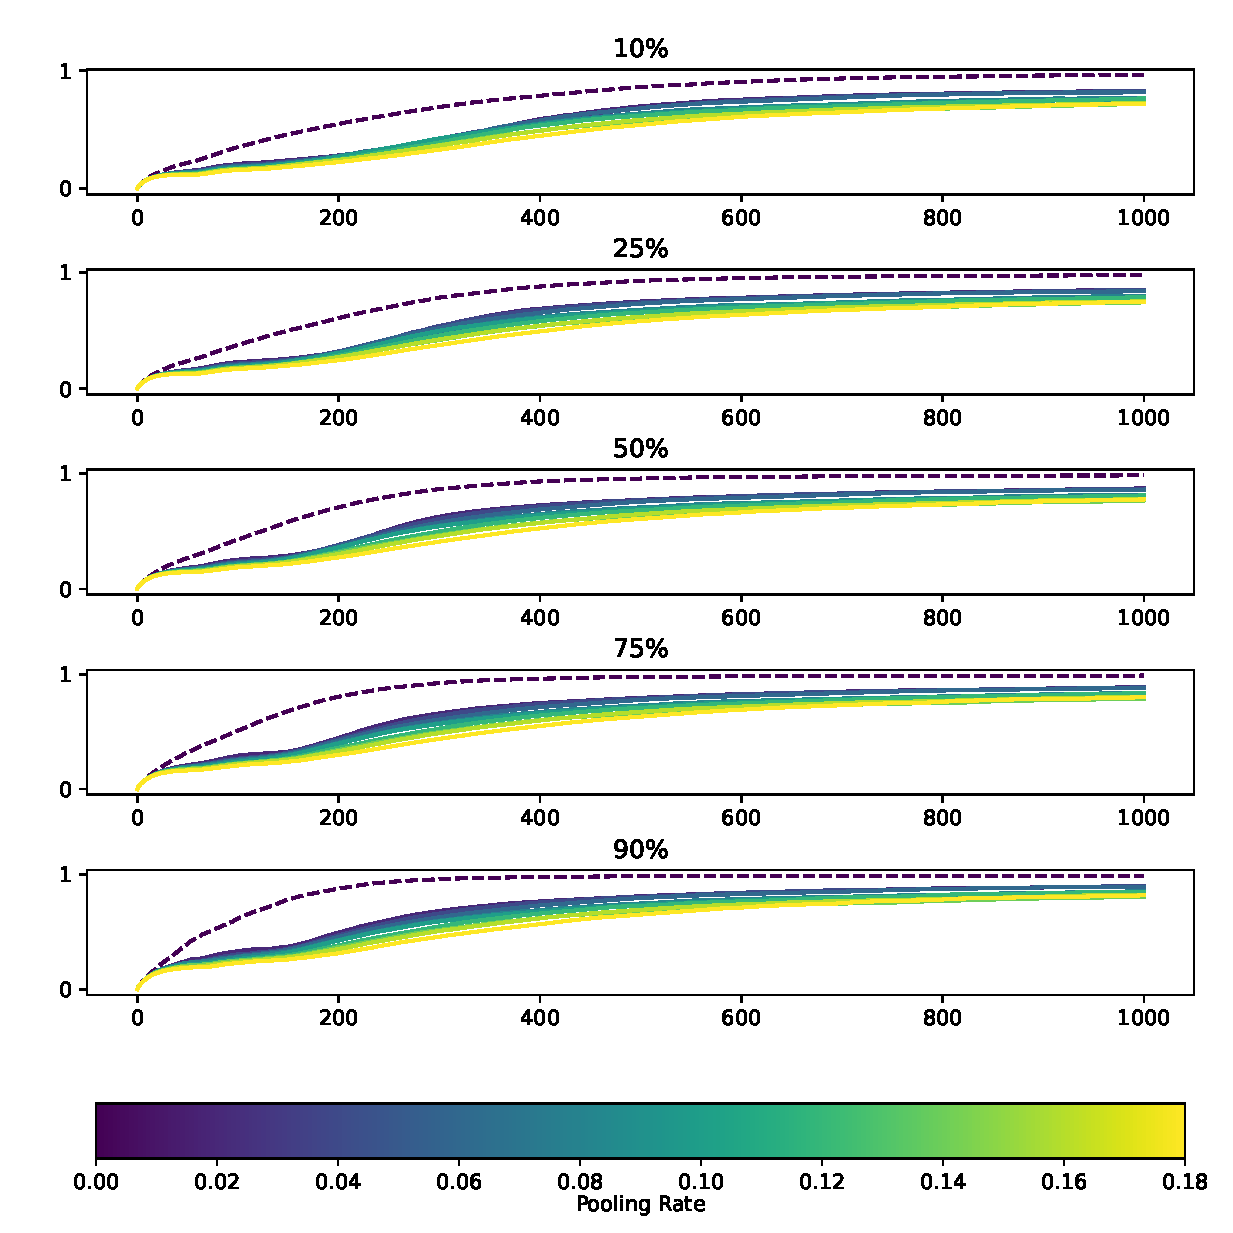
\includegraphics[trim={0cm 0.1cm 0cm 0.3cm}, clip, width=.7\textwidth]{figures/ginis.eps}
%     \caption{Quantiles of Gini coefficients.}
%     \label{fig:ginis}
% \end{figure}

So far we have only looked at a static measure for capital shares, meaning that it can only provide information on the distribution of capital shares, but not which firms are within them. To address this, we follow each firm throughout a simulation and record both the difference between its maximum and minimum rank and the standard deviation of its ranks. Figure \ref{fig:mobility_ridges} demonstrates how the distribution over both of these metrics changes as we increase the pooling rate $\alpha$. Given that there are $N \in \{50, 100, 150 \}$ firms per market, there is an upper limit to the mobility measure. The range shows that even in the no-pooling case the theoretical upper bounds of mobility are reached. However, we observe again that introducing just a small amount of sharing changes the dynamic drastically, as both measures shift completely in their pattern, raising the body of the mobility considerably. In addition, increasing the sharing rate increases the variability of ranks, shifting the distribution to the right. We interpret this as reduced persistence of market positions, a property typically associated with more dynamic competitive environments though our framework does not model competitive interactions explicitly. The baseline case $(\alpha = 0)$ represents pure Gibrat's law dynamics, which are known to produce extreme concentration and lock-in of market leaders \parencite{gibrat1931,sutton1997gibrat}. Any deviation from this baseline through pooling therefore represents an increase in rank mobility, which corresponds to more dynamic competitive conditions. Note that the theoretical maximum of the range metric (equal to $N-1$) is reached even at $\alpha = 0$, but the mass of the distribution shifts rightward with increased pooling, indicating that more firms experience rank mobility rather than just a few outliers. As expected, there is also variability in the response depending on the cost structure, mirroring the sequence of convergence observed above. While simulations based on the power law cost structure reach their maximum mobility for the smallest of $\alpha > 0$, increasing it to higher levels actually decreases mobility slightly, shifting the body of the distribution for both metrics leftwards and increasing spread. 

% Ridge plot for mobility distributions
% This file is \input into the main document

\begin{figure}[htbp]
  \centering
  \begin{tikzpicture}
    \begin{groupplot}[
      group style={
        group size=2 by 1,
        horizontal sep=1cm
      },
      width=0.58\textwidth,
      height=0.75\textheight,
      xlabel style={font=\small},
      ylabel style={font=\small},
      tick label style={font=\scriptsize},
      ytick=\empty,  % No y-ticks for ridge plots
      grid=none,
      % Define plot styles for cost types
      /pgfplots/cost0/.style={color=cost0, fill=cost0, fill opacity=0.5, draw opacity=1},
      /pgfplots/cost1/.style={color=cost1, fill=cost1, fill opacity=0.5, draw opacity=1},
      /pgfplots/cost2/.style={color=cost2, fill=cost2, fill opacity=0.5, draw opacity=1},
      /pgfplots/cost3/.style={color=cost3, fill=cost3, fill opacity=0.5, draw opacity=1},
    ]

    % LEFT PANEL: Rank Ranges
    \nextgroupplot[
      xlabel={Rank Range},
      legend to name=ridgelegend,
      legend columns=4,
      clip=false,
      ymin=-0.5,
      ymax=39.5,
      ytick={0.5,2,3.5,5,6.5,8,9.5,11,12.5,14,15.5,17,18.5,20,21.5,23,24.5,26,27.5,29,30.5,32,33.5,35,36.5,38},
      yticklabels={$\alpha$=0.00,$\alpha$=0.02,$\alpha$=0.04,$\alpha$=0.06,$\alpha$=0.08,$\alpha$=0.10,$\alpha$=0.12,$\alpha$=0.14,$\alpha$=0.16,$\alpha$=0.18,$\alpha$=0.20,$\alpha$=0.22,$\alpha$=0.24,$\alpha$=0.26,$\alpha$=0.28,$\alpha$=0.30,$\alpha$=0.32,$\alpha$=0.34,$\alpha$=0.36,$\alpha$=0.38,$\alpha$=0.40,$\alpha$=0.42,$\alpha$=0.44,$\alpha$=0.46,$\alpha$=0.48,$\alpha$=0.50},
      yticklabel style={font=\scriptsize}
    ]

    % Define ridge spacing parameters (directly in the preamble so they're accessible)
    \pgfmathsetmacro{\ridgeoffset}{1.5}
    \pgfmathsetmacro{\ridgeheight}{1.0}

    % Loop through alpha indices using pgfplotsinvokeforeach (better than foreach for pgfplots)
    \pgfplotsinvokeforeach{0,...,25}{
      % Numeric index (SAFE for math)
      \pgfmathsetmacro{\alphaindex}{#1}
      \pgfmathsetmacro{\ybasenum}{\alphaindex * 1.5}
      \pgfmathsetmacro{\ridgeheightnum}{1.0}

      \pgfmathtruncatemacro{\tmpindex}{\alphaindex}
      \ifnum\tmpindex<10
        \edef\alphafileindex{0\tmpindex}
      \else
        \edef\alphafileindex{\tmpindex}
      \fi

      % Compute alpha value directly (0.00, 0.02, 0.04, ..., 0.50)
      \pgfmathsetmacro{\alphaval}{\alphaindex * 0.02}

      % Cost type 0
      \edef\temp{\noexpand\addplot[cost0, forget plot, fill] table[col sep=comma, header=true, x=x, y expr=\noexpand\thisrow{cost0} * \ridgeheightnum + \ybasenum] {figures/plots/ridge_ranges_alpha\alphafileindex.csv} |- (axis cs:0,\ybasenum) -| cycle;}\temp

      % Cost type 1
      \edef\temp{\noexpand\addplot[cost1, forget plot, fill] table[col sep=comma, header=true, x=x, y expr=\noexpand\thisrow{cost1} * \ridgeheightnum + \ybasenum] {figures/plots/ridge_ranges_alpha\alphafileindex.csv} |- (axis cs:0,\ybasenum) -| cycle;}\temp

      % Cost type 2
      \edef\temp{\noexpand\addplot[cost2, forget plot, fill] table[col sep=comma, header=true, x=x, y expr=\noexpand\thisrow{cost2} * \ridgeheightnum + \ybasenum] {figures/plots/ridge_ranges_alpha\alphafileindex.csv} |- (axis cs:0,\ybasenum) -| cycle;}\temp

      % Cost type 3
      \edef\temp{\noexpand\addplot[cost3, forget plot, fill] table[col sep=comma, header=true, x=x, y expr=\noexpand\thisrow{cost3} * \ridgeheightnum + \ybasenum] {figures/plots/ridge_ranges_alpha\alphafileindex.csv} |- (axis cs:0,\ybasenum) -| cycle;}\temp

    }

    % Add legend entries (using dummy plots)
    \addlegendimage{cost0, mark=square*, only marks}
    \addlegendimage{cost1, mark=square*, only marks}
    \addlegendimage{cost2, mark=square*, only marks}
    \addlegendimage{cost3, mark=square*, only marks}
    \legend{Linear, Quadratic, Power law, Exponential}


    % RIGHT PANEL: Rank Standard Deviation
    \nextgroupplot[
      xlabel={Rank Standard Deviation},
      clip=true,
      ymin=-0.5,
      ymax=39.5,
      ytick=\empty
    ]

    % Loop through alpha indices for std panel
    \pgfplotsinvokeforeach{0,...,25}{
      % Numeric index (safe for math)
      \pgfmathsetmacro{\alphaindex}{#1}
      \pgfmathsetmacro{\ybasenum}{\alphaindex * 1.5}
      \pgfmathsetmacro{\ridgeheightnum}{1.0}

      \pgfmathtruncatemacro{\tmpindex}{\alphaindex}
      \ifnum\tmpindex<10
        \edef\alphafileindex{0\tmpindex}
      \else
        \edef\alphafileindex{\tmpindex}
      \fi

      % Compute alpha value directly (0.00, 0.02, 0.04, ..., 0.50)
      \pgfmathsetmacro{\alphaval}{\alphaindex * 0.02}

      % Cost type 0
      \edef\temp{\noexpand\addplot[cost0, forget plot, fill] table[col sep=comma, header=true, x=x, y expr=\noexpand\thisrow{cost0} * \ridgeheightnum + \ybasenum] {figures/plots/ridge_std_alpha\alphafileindex.csv} |- (axis cs:0,\ybasenum) -| cycle;}\temp

      % Cost type 1
      \edef\temp{\noexpand\addplot[cost1, forget plot, fill] table[col sep=comma, header=true, x=x, y expr=\noexpand\thisrow{cost1} * \ridgeheightnum + \ybasenum] {figures/plots/ridge_std_alpha\alphafileindex.csv} |- (axis cs:0,\ybasenum) -| cycle;}\temp

      % Cost type 2
      \edef\temp{\noexpand\addplot[cost2, forget plot, fill] table[col sep=comma, header=true, x=x, y expr=\noexpand\thisrow{cost2} * \ridgeheightnum + \ybasenum] {figures/plots/ridge_std_alpha\alphafileindex.csv} |- (axis cs:0,\ybasenum) -| cycle;}\temp

      % Cost type 3
      \edef\temp{\noexpand\addplot[cost3, forget plot, fill] table[col sep=comma, header=true, x=x, y expr=\noexpand\thisrow{cost3} * \ridgeheightnum + \ybasenum] {figures/plots/ridge_std_alpha\alphafileindex.csv} |- (axis cs:0,\ybasenum) -| cycle;}\temp

    }

    \end{groupplot}

    % Place legend below both plots, centered
    \node at ($(group c1r1.south)!0.5!(group c2r1.south) - (0,1.5cm)$) [anchor=north] {%
      \pgfplotslegendfromname{ridgelegend}%
    };

  \end{tikzpicture}
  \caption{Mobility distributions across profit-sharing levels. Each ridge represents a different $\alpha$ level, with distributions overlaid for all four cost function types. Left panel shows the distribution of rank ranges (maximum minus minimum rank), while the right panel shows rank standard deviation. Higher values indicate greater firm mobility within markets.}
  \label{fig:mobility_ridges}
\end{figure}


\section{Discussion}
\label{sec:Discussion}
A recurring theme in the search for determinants of conglomerate formation is diversification to mitigate risks. As specialization of the Smithian \parencite{smith1776inquiry} and Ricardian \parencite{ricardo1817principles} nature allows us to increase our efficiency, and as we have steadily increased the degree of roundaboutness of production through capital intensification \parencite{bawerk1921kapital}, the potential downsides from miscalculation or shocks loom ever larger. Mitigating these, however, is also becoming simpler \parencite{felton1971conglomerate}, as both internal and external means of diversification \parencite{goldberg1973effect} are available, with their relative attractiveness depending on context. As demonstrated above, \textit{cooperative diversification} from conglomerate formation offers a reliable mitigation pathway and is applicable to many risk vectors. \par
Among these are macroeconomic or political shocks that are specific to certain geographic regions or sectors of the economy. The literature on international trade has picked up this theme arguing that cross-country foreign direct investment reduces country-specific risks \parencite{ramondo2010role} and even increases between less correlated markets \parencite{ramondo2013proximity}. Similarly, \textcite{amit1988concept} argue that conglomeration can diversify across business cycles, while \textcite{audretsch1989determinants} proposes that it can even be used to match different product life cycles. \par
Our model assumes independence of growth increments across markets, which maximizes the pooling benefit. In practice, markets exhibit varying degrees of correlation, particularly during economic crises when correlations tend to spike \parencite{forbes2002no}. \textcite{peters2022ergodicity} show that positive correlation reduces but does not eliminate pooling benefits, unless they are perfectly correlated. Our results therefore represent an upper bound on the incentives for conglomerate formation. This has two implications: first, conglomerates will preferentially form across markets with lower correlation structures; second, the competitive effects we identify will be attenuated in highly correlated environments. Empirically observed conglomerate formation rates and concentration effects should therefore be expected to be weaker than our simulations imply, particularly in periods or sectors with elevated cross-market correlations. \par
Our results shed light on the longstanding diversification discount debate. Early findings suggest that diversified firms trade at a discount relative to focused firms \parencite{lang1994tobins, berger1995diversification}, which has been taken as evidence that conglomeration destroys value. However, this evidence has been substantially challenged on methodological grounds: \textcite{campa2002explaining} show that the discount largely reflects endogeneity, and \textcite{villalonga2004diversification} finds a diversification premium when measurement biases are corrected. Our simulation results offer a structural interpretation. The non-linear relationship between pooling rate $\alpha$ and conglomerate outcomes, which is persistent across all our findings, implies that the value of conglomeration is non-monotonic: moderate pooling enhances growth rates for all constituent firms, but excessive pooling combined with coordination costs $\Phi(O_c)$ erodes these gains. This means that the diversification discount and premium can coexist in the same economy. Conglomerates that pool at rates near the optimum achieve higher time-average growth rates. Most telling for our framework, \textcite{kuppuswamy2016does} document that the diversification discount reversed during the 2007--2009 financial crisis, when conglomerates maintained access to internal capital while focused firms faced external financing constraints. This is precisely the setting where pooling benefits under multiplicative dynamics should manifest most strongly---when external options are limited and the variance drain on growth rates becomes the binding constraint. \par
A related point concerns the role of agency costs. The internal capital markets literature has documented how divisional rent-seeking corrupts capital allocation \parencite{scharfstein2000dark}, how headquarters with limited power misallocate capital across divisions \parencite{rajan2000cost}, and how free cash flow enables empire-building by self-interested managers \parencite{jensen1986agency}. These are real frictions. However, having seen the model, the reader will note that the coordination costs $\Phi(O_c)$ in Equations \ref{eq:power_law}--\ref{eq:exponential} capture the real resource costs of managing a larger organization in the tradition of \textcite{coase19883} and \textcite{williamson1967hierarchical}, which include the costs of communication, monitoring, and bureaucratic overhead that increase with conglomerate scope. These are conceptually distinct from agency costs, which arise from misaligned incentives between managers and shareholders. Our model deliberately abstracts from the latter. By showing that an intrinsic growth synergy from pooling exists even in the complete absence of agency problems, we establish a benchmark: the mathematical benefits of variance reduction under compounding are present regardless of governance quality. Agency costs then determine how much of this potential is realized in practice. The crisis evidence of \textcite{kuppuswamy2016does} is consistent with this interpretation, suggesting that survival pressures during crises align managerial and shareholder incentives, allowing the underlying pooling benefits to become visible. \par
The sensitivity of our results to the cost function specification (Figures \ref{fig:metrics}--\ref{fig:market_shares}) is itself informative. Power law costs, which scale initially slowly, permit larger but fewer conglomerates that reach their mobility ceiling at lower pooling rates. Exponential costs, by contrast, impose steep penalties on size, producing more numerous but smaller conglomerates with a wider effective range of $\alpha$. This suggests an empirically testable prediction: industries where coordination costs scale slowly with scope (e.g., financial holding companies managing independent portfolio firms) should exhibit fewer, larger conglomerates, while industries with rapidly scaling coordination costs (e.g., manufacturing with tightly coupled supply chains) should exhibit more, smaller ones. The fact that the direction of the pooling effect on concentration and mobility is robust across all four cost specifications, while the magnitude varies, indicates that the mechanism we identify is general even though the optimal conglomerate size is context-dependent. \par
A striking feature of our results is the discontinuity at $\alpha = 0$. Even minimal pooling fundamentally alters market dynamics away from the extreme concentration produced by pure Gibrat dynamics (Figure \ref{fig:market_shares}). Under the baseline of no pooling, multiplicative growth produces winner-take-all outcomes where a single firm absorbs nearly the entire market. This is the known consequence of random multiplicative processes \parencite{gibrat1931, gabaix1999zipf}. The introduction of any positive pooling rate breaks this dynamic, raising capital shares for lower quantiles and compressing inequality. The practical implication is that even loose conglomerate structures with modest internal resource transfers may be sufficient to generate the pro-competitive effects we document. This is consistent with the observation that venture capital firms enforce low pooling rates for their portfolio companies and incubator batches \parencite{boyd2023ergodic}, achieving meaningful variance reduction without heavy coordination overhead. More broadly, the pooling mechanism applies to any multiplicative process, extending beyond financial capital to physical and human capital, reputation, and other resources of interest to economic inquiry \parencite{pietronero2001explaining, sibani2020human}. 

\textcite{lewellen1971pure} offers a purely financial rationale for conglomeration, where firms merge in order to mitigate financing frictions and to provide internal capital markets \parencite{boguth2022dissecting}. Our results allow a sharper distinction between this coinsurance channel and the multiplicative dynamics mechanism. The coinsurance rationale operates through a static distributional effect---combining imperfectly correlated cash flows enhances debt capacity. The mechanism we identify operates through temporal compounding as formalized in Equation \ref{eq:pooling_improvement}: variance reduction directly increases the geometric growth rate of equity over time, independent of leverage effects. The two channels are complementary, but the growth-rate channel we document persists even when firms face no financing frictions. In addition, pooling can be used to reduce the highly volatile returns inherent to R\&D efforts, or share the costs associated with them \parencite{felton1971conglomerate}. 

The mechanism we identify operates alongside several other forces that govern organizational form. Selection determines which firms become conglomerates in the first place; managerial agency frictions can corrupt the internal capital reallocation that makes pooling effective; operational integration generates synergies that our model does not capture; market correlations attenuate the pooling benefit; and broader institutional context shapes the costs of coordination across borders, regulatory regimes, and ownership structures. Each of these forces operates simultaneously with the pooling mechanism, and the observed organizational form of any particular conglomerate reflects their joint operation. Our contribution is to isolate and characterize one of these forces under explicit assumptions. The crisis evidence of \textcite{kuppuswamy2016does} is suggestive of contexts where the pooling channel becomes more visible; systematic identification across non-crisis settings would require considerably more demanding empirical work than the existing literature provides.

We emphasize that our model speaks to market structure outcomes rather than welfare. While reduced concentration is often associated with improved consumer welfare in standard models, this connection requires assumptions about pricing, demand, and allocative efficiency that our framework does not incorporate. The welfare implications of the dynamics we identify therefore remain an open question, requiring models that integrate our growth-rate-optimization mechanism with explicit market interactions and a stance on the appropriate welfare criterion.

\section{Conclusion}
\label{sec:Conclusion}
This article has developed a novel theoretical foundation for conglomerate mergers grounded in multiplicative dynamics and time-average growth-rate optimization. Building on the cooperation framework of \textcite{peters2022ergodicity}, who show that resource pooling is positive-sum under multiplicative dynamics, we have demonstrated that this mechanism provides a distinct rationale for conglomerate merger formation. By embedding their pooling result within an agent-based model of endogenous merger decisions, we show that growth-rate optimization through variance reduction can explain conglomerate formation even absent economies of scale, market power, tax motivations, or management incentive considerations — and that acting on these incentives compresses capital share distributions and increases rank mobility. Unlike portfolio diversification, which reduces a shareholder's risk exposure while leaving each firm's growth trajectory unchanged, cooperative diversification through pooling directly improves the growth dynamics of constituent firms. This extends and reinterprets the risk-reduction arguments of \textcite{amihud1981risk}, \textcite{lewellen1971pure}, and \textcite{mueller1969theory} within the framework appropriate for multiplicative processes, and complements the internal capital markets literature \parencite{stein1997internal, gertner1994internal} by identifying a growth-rate channel that operates even absent information asymmetries or financing frictions. 

Our simulations characterize the implications of the pooling mechanism under the assumption that firms act on the merger incentives it generates: capital share distributions compress across all quantiles, rank mobility increases, and the persistence of market dominance that characterizes pure multiplicative growth is reduced. The relationship between pooling and market outcomes is non-monotonic, while coordination costs impose a natural limit on conglomerate scope, producing an optimal pooling rate that depends on the cost structure. This non-monotonicity offers a model-based interpretation of the heterogeneous empirical evidence on the diversification discount \parencite{lang1994tobins, berger1995diversification, campa2002explaining, villalonga2004diversification}: conglomerates near the optimum implied by our model achieve higher time-average growth rates, while those that overshoot or face steep coordination costs do not. The robustness of the concentration-reducing and mobility-increasing direction across all four cost specifications, combined with the sensitivity of magnitude to cost structure, suggests that the mechanism is general even though its quantitative implications are context-dependent. 

Several avenues for future work present themselves. First, incorporating a pricing mechanism would allow for statements on consumer welfare, which our current framework, focused on market structure, cannot provide. Second, we assume normally distributed growth increments, whereas firm growth is empirically heavy-tailed \parencite{lahr2023fat, stanley1996scaling}, with negative shocks occurring more frequently than normality predicts \parencite{cont2001empirical, viscusi2014shifting}. Since large negative realizations have an outsized impact on the growth rate under multiplicative dynamics, fat-tailed distributions would likely strengthen the case for pooling, making it a natural extension. Finally, our assumption of uncorrelated markets represents an upper bound on pooling benefits. Empirically testing whether conglomerate mergers are more common across industries with lower return correlations, and whether conglomerate size distributions match the predictions of specific cost function shapes, would provide informative tests of the framework's predictions. The pooling mechanism we characterize is one among several forces governing organizational form. Selection, agency frictions, operational synergies, market correlations, and institutional context all enter the determination of equilibrium outcomes. Isolating the empirical signature of the pooling channel specifically remains a demanding identification problem, which we leave to subsequent work.

\section*{Acknowledgments}
Calculations were performed using the festus-cluster of the Bayreuth Centre for High Performance Computing (\url{https://www.bzhpc.uni-bayreuth.de}), funded by the Deutsche Forschungsgemeinschaft (DFG, German Research Foundation) -- 523317330.

\section*{Code and data availability}
The simulation code and replication materials for this paper are publicly available at \href{https://github.com/SimonBloethner/conglomerates}{https://github.com/SimonBloethner/conglomerates}. The package includes the agent-based model implementation, calibrated parameter values for all cost-function specifications, and scripts to reproduce all figures and tables in the paper.



\clearpage


\printbibliography




\end{document}